% lecture10_ro.tex -- GENERATED by build_L10.py from L10_numbers.json; do not edit by hand.
\documentclass[10pt,aspectratio=169,t]{beamer}
% =============================================================================
% nn_preamble.tex -- shared Beamer preamble of Neural Networks and Deep Learning (NN)
% Used by every lecture: lectures/Lk/lecturek.tex does
%   \documentclass[10pt,aspectratio=169,t]{beamer}
%   % =============================================================================
% nn_preamble.tex -- shared Beamer preamble of Neural Networks and Deep Learning (NN)
% Used by every lecture: lectures/Lk/lecturek.tex does
%   \documentclass[10pt,aspectratio=169,t]{beamer}
%   % =============================================================================
% nn_preamble.tex -- shared Beamer preamble of Neural Networks and Deep Learning (NN)
% Used by every lecture: lectures/Lk/lecturek.tex does
%   \documentclass[10pt,aspectratio=169,t]{beamer}
%   \input{../common/nn_preamble}
%   \nnlecture{k}{Lecture title}
% Logos live in lectures/common/logos/, charts in lectures/Lk/charts/.
% Do NOT add \hfuzz / \vfuzz / \hbadness here: overfull boxes must be fixed, not hidden.
% =============================================================================

\usetheme{default}
\setbeamersize{text margin left=7mm, text margin right=7mm}

% ---------------------------------------------------------------- packages
\usepackage[utf8]{inputenc}
\usepackage[T1]{fontenc}
\usepackage{lmodern}
\usepackage{amsmath, amssymb}
\usepackage{mathtools}
\usepackage{bm}
\usepackage{tikz}
\usetikzlibrary{arrows.meta, positioning, calc, shapes.misc}
\usepackage{booktabs}
\usepackage{array}
\usepackage{graphicx}
\usepackage{colortbl}
\usepackage{xcolor}
\usepackage{multicol}
\hypersetup{colorlinks=true, linkcolor=MainBlue, urlcolor=MainBlue, citecolor=MainBlue}
\graphicspath{{../common/logos/}}   % charts are included with their language folder: charts/en/, charts/ro/

% ---------------------------------------------------------------- colours
\definecolor{MainBlue}{RGB}{26, 58, 110}
\definecolor{IDAred}{RGB}{205, 0, 0}
\definecolor{DarkGray}{RGB}{51, 51, 51}
\definecolor{FooterGray}{RGB}{100, 100, 100}
\definecolor{BlockGray}{RGB}{236, 238, 242}
\definecolor{KeynoteGray}{RGB}{218, 218, 218}
\definecolor{Crimson}{RGB}{190, 40, 50}
\definecolor{Forest}{RGB}{30, 110, 50}
\definecolor{Bitter}{RGB}{214, 150, 20}
% chart palette (same hex values and order as lectures/common/nn_plot.py SERIES)
\definecolor{Ser1}{HTML}{2A78D6}
\definecolor{Ser2}{HTML}{EB6834}
\definecolor{Ser3}{HTML}{1BAF7A}
\definecolor{Ser4}{HTML}{EDA100}
\definecolor{Ser5}{HTML}{E87BA4}
\definecolor{Ser6}{HTML}{008300}
\definecolor{Ser7}{HTML}{6250D6}
\definecolor{Ser8}{HTML}{E34948}

\setbeamertemplate{background}{%
  \begin{tikzpicture}[remember picture, overlay]
    \shade[shading=axis, shading angle=315, top color=white, bottom color=KeynoteGray]
      (current page.south west) rectangle (current page.north east);
  \end{tikzpicture}}
\setbeamercolor{background canvas}{bg=}
\setbeamercolor{structure}{fg=MainBlue}
\setbeamercolor{normal text}{fg=DarkGray}
\setbeamercolor{title}{fg=IDAred}
\setbeamercolor{frametitle}{fg=IDAred, bg=}
\setbeamercolor{block title}{bg=MainBlue, fg=white}
\setbeamercolor{block body}{bg=BlockGray, fg=DarkGray}
\setbeamercolor{block title alerted}{bg=Crimson, fg=white}
\setbeamercolor{block body alerted}{bg=Crimson!7, fg=DarkGray}
\setbeamercolor{block title example}{bg=Forest, fg=white}
\setbeamercolor{block body example}{bg=Forest!7, fg=DarkGray}
\setbeamercolor{item}{fg=MainBlue}
\setbeamerfont{frametitle}{size=\large, series=\bfseries}
\setbeamerfont{block title}{size=\small, series=\bfseries}
\setbeamertemplate{blocks}[rounded][shadow=false]
\setbeamertemplate{itemize item}{\color{MainBlue}$\boxdot$}
\setbeamertemplate{itemize subitem}{\color{MainBlue}\scriptsize$\blacktriangleright$}
% compact two-level lists: level 1 = main point, level 2 = details (no text outside bullets)
\setbeamerfont{itemize/enumerate subbody}{size=\footnotesize}
\setlength{\leftmargini}{1.1em}
\setlength{\leftmarginii}{1.1em}
\setbeamertemplate{itemize/enumerate body begin}{\setlength{\topsep}{0pt}\setlength{\partopsep}{0pt}\setlength{\parskip}{0pt}}
\setbeamertemplate{itemize/enumerate subbody begin}{\setlength{\topsep}{0pt}\setlength{\partopsep}{0pt}\setlength{\itemsep}{0pt}\vspace{-0.4ex}}

\setbeamertemplate{enumerate item}{\color{MainBlue}\insertenumlabel.}
\setlength{\leftmargini}{1.3em}
\setlength{\leftmarginii}{1.2em}
\setbeamertemplate{navigation symbols}{}
\setbeamertemplate{section in toc}{\color{MainBlue}$\blacktriangleright$~\inserttocsection}
\setbeamertemplate{caption}{\raggedright\insertcaption\par}
% frame subtitle = precise citation line under the claim title (Weron style)
\setbeamerfont{framesubtitle}{size=\footnotesize}
\setbeamercolor{framesubtitle}{fg=FooterGray}
% outline that reappears at every section with the current section highlighted
\setbeamertemplate{section in toc shaded}[default][35]
\setbeamertemplate{subsection in toc shaded}[default][35]
\setbeamertemplate{subsection in toc}{\leavevmode\leftskip=2.2em\color{DarkGray}\small\inserttocsubsection\par}
\AtBeginSection[]{{\begin{frame}{\txtoutline}\vspace{2mm}\small
  \tableofcontents[currentsection,hideothersubsections]\end{frame}}}

% ---------------------------------------------------------------- head and foot
\setbeamertemplate{headline}{%
  \vskip10pt%
  \hbox to \paperwidth{\hskip0.5cm%
    {\small\color{FooterGray}\renewcommand{\hyperlink}[2]{##2}\insertsectionhead}%
    \hfill\textcolor{FooterGray}{\small\insertframenumber}\hskip0.5cm}%
  \vskip4pt{\color{FooterGray}\hrule height 0.4pt}}
% footer as in the other courses (MFM, SFM): course name on the left, small sparkline on the right
\setbeamertemplate{footline}{%
  {\color{FooterGray}\hrule height 0.4pt}\vskip4pt%
  \hbox to \paperwidth{\hskip0.5cm%
    \textcolor{FooterGray}{\small\txtcourse}%
    \hfill\raisebox{-0.1em}{\begin{tikzpicture}[x=0.08em, y=0.08em, line width=0.4pt]
      \draw[FooterGray] (0,3) -- (1,4) -- (2,3.5) -- (3,5) -- (4,4) -- (5,6) -- (6,5.5) -- (7,4) -- (8,5) -- (9,7) -- (10,6) -- (11,5) -- (12,6.5) -- (13,8) -- (14,7) -- (15,6) -- (16,7.5) -- (17,9) -- (18,8) -- (19,7) -- (20,8.5) -- (21,10) -- (22,9) -- (23,8) -- (24,9.5);
    \end{tikzpicture}}\hskip0.5cm}%
  \vskip6pt}

% ---------------------------------------------------------------- title page
\defbeamertemplate*{title page}{nn}[1][]{%
  \vspace{0.15cm}
  \begin{center}
    \href{https://www.ase.ro}{
\includegraphics[height=0.9cm]{ase_logo.png}}\hspace{0.3cm}%
    \href{https://ipe.ro/new}{
\includegraphics[height=0.9cm]{acad_logo.png}}\hspace{0.3cm}%
    \href{https://theida.net}{
\includegraphics[height=0.9cm]{ida_logo.png}}\hspace{0.3cm}%
    \href{https://blockchain-research-center.com}{
\includegraphics[height=0.9cm]{brc_logo.png}}\hspace{0.3cm}%
    \href{https://www.ai4efin.ase.ro}{
\includegraphics[height=0.9cm]{ai4efin_logo.png}}\hspace{0.3cm}%
    \href{https://www.digital-finance-msca.com}{
\includegraphics[height=0.9cm]{msca_logo.png}}%
  \end{center}
  \vspace{0.45cm}
  \begin{center}
    \begin{minipage}{0.1\textwidth}\centering
      \href{https://quantlet.com}{
\includegraphics[height=0.9cm]{ql_logo.png}}\end{minipage}%
    \begin{minipage}{0.78\textwidth}\centering
      {\Large\bfseries\usebeamercolor[fg]{title}\inserttitle}\par\vspace{0.25cm}
      {\large\usebeamercolor[fg]{title}\insertsubtitle}\end{minipage}%
    \begin{minipage}{0.1\textwidth}\centering
      \href{https://quantinar.com}{
\includegraphics[height=0.9cm]{qr_logo.png}}\end{minipage}
  \end{center}
  \vfill
  \hspace{0.4cm}{\bfseries\insertauthor}\par\vspace{0.12cm}
  \hspace{0.4cm}\begin{minipage}[t]{0.92\textwidth}\raggedright\footnotesize\insertinstitute\end{minipage}
  \par\vspace{0.4cm}}

% ---------------------------------------------------------------- lecture metadata
\newcommand{\nnshort}{}
\newcommand{\nnnb}{notebooks}
\newcommand{\nnrepo}{https://github.com/danpele/NEURAL_BIZ/tree/main}
% language-dependent labels (English default; \nnromanian switches to Romanian, call it before \nnlecture)
\newcommand{\txtcourse}{Neural Networks and Deep Learning}
\newcommand{\txtlecture}{Lecture}
\newcommand{\txtoutline}{Outline}
\newcommand{\txtintuition}{In one sentence:}
\newcommand{\txtjob}{In practice:}
\newcommand{\txttry}{Experiment yourself:}
\newcommand{\txtwhere}{where}
\newcommand{\txtsim}{SIMULATED DATA (teaching illustration)}
\newcommand{\txtnbsuffix}{}
\newcommand{\txtinstitute}{Bucharest University of Economic Studies (ASE), Department of Statistics and Econometrics\\
    Romanian Academy, Institute for Economic Forecasting (IPE)\\
    IDA Institute Digital Assets \textbullet\ AI4EFin \textbullet\ MSCA Digital Finance}
\newcommand{\nnromanian}{%
  \renewcommand{\txtcourse}{Rețele neuronale și deep learning}%
  \renewcommand{\txtlecture}{Cursul}%
  \renewcommand{\txtoutline}{Cuprins}%
  \renewcommand{\txtintuition}{Pe scurt:}%
  \renewcommand{\txtjob}{În practică:}%
  \renewcommand{\txttry}{Exercițiu practic:}%
  \renewcommand{\txtwhere}{unde}%
  \renewcommand{\txtsim}{DATE SIMULATE (doar pentru ilustrare)}%
  \renewcommand{\txtnbsuffix}{\string_ro}%
  \renewcommand{\txtinstitute}{Academia de Studii Economice din București (ASE), Departamentul de Statistică și Econometrie\\
    Academia Română, Institutul de Prognoză Economică (IPE)\\
    IDA Institute Digital Assets \textbullet\ AI4EFin \textbullet\ MSCA Digital Finance}}
\newcommand{\nnlecture}[2]{%
  \renewcommand{\nnshort}{\txtlecture\ #1}%
  \renewcommand{\nnnb}{notebooks/L#1\string_notebook\txtnbsuffix.ipynb}%
  \title[NN]{\txtcourse}%
  \subtitle{\txtlecture\ #1: #2}%
  \author{Prof.\ dr.\ Daniel Traian PELE}%
  \institute{\txtinstitute}%
  \date{}}

% ---------------------------------------------------------------- teaching blocks (one message per frame)
% \intuition{one plain sentence}  ->  formula with every symbol defined  ->  real-data example  ->  \manager{one line}
\newcommand{\intuition}[1]{\begin{itemize}\item {\color{MainBlue}\textbf{\txtintuition}}~#1\end{itemize}\vspace{0.6mm}}
\newcommand{\manager}[1]{\colorbox{Forest!10}{\parbox{\dimexpr\linewidth-2\fboxsep\relax}{\footnotesize
  \begin{itemize}\setlength{\itemsep}{0pt}\item \textbf{\color{Forest}\txtjob}~#1\end{itemize}}}}
% Experiment yourself: pointer to the matching notebook section
\newcommand{\tryit}[1]{{\scriptsize\href{\nnrepo/\nnnb}{%
  \raisebox{-0.15em}{
\includegraphics[height=0.85em]{ql_logo.png}}\,\textbf{\txttry}~\color{MainBlue}#1}}}
% bottom row: manager line (left) + experiment pointer (right), pinned to the bottom of the frame
\newcommand{\bottomrow}[2]{\par\vfill\noindent\begin{minipage}[b]{0.72\linewidth}#1\end{minipage}\hfill
  \begin{minipage}[b]{0.26\linewidth}\raggedleft #2\end{minipage}\par\vspace{0.5mm}}
\newcommand{\where}[1]{{\footnotesize\textbf{\txtwhere}~#1\par}}

% ---------------------------------------------------------------- helpers
% chart source line under a figure: \chartsource{Source ...; period ...}
\newcommand{\chartsource}[1]{\par\vspace{1pt}{\scriptsize\color{FooterGray}#1\par}}
% link to code: \quantlet{label}{path inside the repo}
\newcommand{\quantlet}[2]{\par\vspace{1pt}\hfill\href{\nnrepo/#2}{%
  \raisebox{-0.15em}{
\includegraphics[height=0.75em]{ql_logo.png}}\textcolor{MainBlue}{\scriptsize\ #1}}}
% inline Quantlet link for the bottom-right corner of a frame: \qlink{label}{path inside the repo}
\newcommand{\qlink}[2]{{\scriptsize\href{\nnrepo/#2}{\raisebox{-0.15em}{
\includegraphics[height=0.85em]{ql_logo.png}}\,\textcolor{MainBlue}{#1}}}}
\newcommand{\simlabel}{\colorbox{Crimson!12}{\scriptsize\bfseries\color{Crimson}\txtsim}}
\newcommand{\E}{\mathbb{E}}
\newcommand{\Var}{\operatorname{Var}}
\newcommand{\Cov}{\operatorname{Cov}}
\newcommand{\Corr}{\operatorname{Corr}}
\newcommand{\asinh}{\operatorname{asinh}}
\newcommand{\iid}{\overset{\text{i.i.d.}}{\sim}}
\newcommand{\EUR}{EUR}
% deep-learning notation (Bishop & Bishop, 2024): vectors bold lower case, matrices bold upper case
\newcommand{\R}{\mathbb{R}}
\newcommand{\vx}{\mathbf{x}}
\newcommand{\vy}{\mathbf{y}}
\newcommand{\vz}{\mathbf{z}}
\newcommand{\vh}{\mathbf{h}}
\newcommand{\vw}{\mathbf{w}}
\newcommand{\vb}{\mathbf{b}}
\newcommand{\mW}{\mathbf{W}}
\newcommand{\mX}{\mathbf{X}}
\newcommand{\btheta}{\boldsymbol{\theta}}
\newcommand{\loss}{\mathcal{L}}
\newcommand{\dataset}{\mathcal{D}}
\DeclareMathOperator*{\argmin}{arg\,min}
\DeclareMathOperator*{\argmax}{arg\,max}
\DeclareMathOperator{\softmax}{softmax}
\DeclareMathOperator{\ReLU}{ReLU}
\DeclareMathOperator{\sigm}{\sigma}

%   \nnlecture{k}{Lecture title}
% Logos live in lectures/common/logos/, charts in lectures/Lk/charts/.
% Do NOT add \hfuzz / \vfuzz / \hbadness here: overfull boxes must be fixed, not hidden.
% =============================================================================

\usetheme{default}
\setbeamersize{text margin left=7mm, text margin right=7mm}

% ---------------------------------------------------------------- packages
\usepackage[utf8]{inputenc}
\usepackage[T1]{fontenc}
\usepackage{lmodern}
\usepackage{amsmath, amssymb}
\usepackage{mathtools}
\usepackage{bm}
\usepackage{tikz}
\usetikzlibrary{arrows.meta, positioning, calc, shapes.misc}
\usepackage{booktabs}
\usepackage{array}
\usepackage{graphicx}
\usepackage{colortbl}
\usepackage{xcolor}
\usepackage{multicol}
\hypersetup{colorlinks=true, linkcolor=MainBlue, urlcolor=MainBlue, citecolor=MainBlue}
\graphicspath{{../common/logos/}}   % charts are included with their language folder: charts/en/, charts/ro/

% ---------------------------------------------------------------- colours
\definecolor{MainBlue}{RGB}{26, 58, 110}
\definecolor{IDAred}{RGB}{205, 0, 0}
\definecolor{DarkGray}{RGB}{51, 51, 51}
\definecolor{FooterGray}{RGB}{100, 100, 100}
\definecolor{BlockGray}{RGB}{236, 238, 242}
\definecolor{KeynoteGray}{RGB}{218, 218, 218}
\definecolor{Crimson}{RGB}{190, 40, 50}
\definecolor{Forest}{RGB}{30, 110, 50}
\definecolor{Bitter}{RGB}{214, 150, 20}
% chart palette (same hex values and order as lectures/common/nn_plot.py SERIES)
\definecolor{Ser1}{HTML}{2A78D6}
\definecolor{Ser2}{HTML}{EB6834}
\definecolor{Ser3}{HTML}{1BAF7A}
\definecolor{Ser4}{HTML}{EDA100}
\definecolor{Ser5}{HTML}{E87BA4}
\definecolor{Ser6}{HTML}{008300}
\definecolor{Ser7}{HTML}{6250D6}
\definecolor{Ser8}{HTML}{E34948}

\setbeamertemplate{background}{%
  \begin{tikzpicture}[remember picture, overlay]
    \shade[shading=axis, shading angle=315, top color=white, bottom color=KeynoteGray]
      (current page.south west) rectangle (current page.north east);
  \end{tikzpicture}}
\setbeamercolor{background canvas}{bg=}
\setbeamercolor{structure}{fg=MainBlue}
\setbeamercolor{normal text}{fg=DarkGray}
\setbeamercolor{title}{fg=IDAred}
\setbeamercolor{frametitle}{fg=IDAred, bg=}
\setbeamercolor{block title}{bg=MainBlue, fg=white}
\setbeamercolor{block body}{bg=BlockGray, fg=DarkGray}
\setbeamercolor{block title alerted}{bg=Crimson, fg=white}
\setbeamercolor{block body alerted}{bg=Crimson!7, fg=DarkGray}
\setbeamercolor{block title example}{bg=Forest, fg=white}
\setbeamercolor{block body example}{bg=Forest!7, fg=DarkGray}
\setbeamercolor{item}{fg=MainBlue}
\setbeamerfont{frametitle}{size=\large, series=\bfseries}
\setbeamerfont{block title}{size=\small, series=\bfseries}
\setbeamertemplate{blocks}[rounded][shadow=false]
\setbeamertemplate{itemize item}{\color{MainBlue}$\boxdot$}
\setbeamertemplate{itemize subitem}{\color{MainBlue}\scriptsize$\blacktriangleright$}
% compact two-level lists: level 1 = main point, level 2 = details (no text outside bullets)
\setbeamerfont{itemize/enumerate subbody}{size=\footnotesize}
\setlength{\leftmargini}{1.1em}
\setlength{\leftmarginii}{1.1em}
\setbeamertemplate{itemize/enumerate body begin}{\setlength{\topsep}{0pt}\setlength{\partopsep}{0pt}\setlength{\parskip}{0pt}}
\setbeamertemplate{itemize/enumerate subbody begin}{\setlength{\topsep}{0pt}\setlength{\partopsep}{0pt}\setlength{\itemsep}{0pt}\vspace{-0.4ex}}

\setbeamertemplate{enumerate item}{\color{MainBlue}\insertenumlabel.}
\setlength{\leftmargini}{1.3em}
\setlength{\leftmarginii}{1.2em}
\setbeamertemplate{navigation symbols}{}
\setbeamertemplate{section in toc}{\color{MainBlue}$\blacktriangleright$~\inserttocsection}
\setbeamertemplate{caption}{\raggedright\insertcaption\par}
% frame subtitle = precise citation line under the claim title (Weron style)
\setbeamerfont{framesubtitle}{size=\footnotesize}
\setbeamercolor{framesubtitle}{fg=FooterGray}
% outline that reappears at every section with the current section highlighted
\setbeamertemplate{section in toc shaded}[default][35]
\setbeamertemplate{subsection in toc shaded}[default][35]
\setbeamertemplate{subsection in toc}{\leavevmode\leftskip=2.2em\color{DarkGray}\small\inserttocsubsection\par}
\AtBeginSection[]{{\begin{frame}{\txtoutline}\vspace{2mm}\small
  \tableofcontents[currentsection,hideothersubsections]\end{frame}}}

% ---------------------------------------------------------------- head and foot
\setbeamertemplate{headline}{%
  \vskip10pt%
  \hbox to \paperwidth{\hskip0.5cm%
    {\small\color{FooterGray}\renewcommand{\hyperlink}[2]{##2}\insertsectionhead}%
    \hfill\textcolor{FooterGray}{\small\insertframenumber}\hskip0.5cm}%
  \vskip4pt{\color{FooterGray}\hrule height 0.4pt}}
% footer as in the other courses (MFM, SFM): course name on the left, small sparkline on the right
\setbeamertemplate{footline}{%
  {\color{FooterGray}\hrule height 0.4pt}\vskip4pt%
  \hbox to \paperwidth{\hskip0.5cm%
    \textcolor{FooterGray}{\small\txtcourse}%
    \hfill\raisebox{-0.1em}{\begin{tikzpicture}[x=0.08em, y=0.08em, line width=0.4pt]
      \draw[FooterGray] (0,3) -- (1,4) -- (2,3.5) -- (3,5) -- (4,4) -- (5,6) -- (6,5.5) -- (7,4) -- (8,5) -- (9,7) -- (10,6) -- (11,5) -- (12,6.5) -- (13,8) -- (14,7) -- (15,6) -- (16,7.5) -- (17,9) -- (18,8) -- (19,7) -- (20,8.5) -- (21,10) -- (22,9) -- (23,8) -- (24,9.5);
    \end{tikzpicture}}\hskip0.5cm}%
  \vskip6pt}

% ---------------------------------------------------------------- title page
\defbeamertemplate*{title page}{nn}[1][]{%
  \vspace{0.15cm}
  \begin{center}
    \href{https://www.ase.ro}{
\includegraphics[height=0.9cm]{ase_logo.png}}\hspace{0.3cm}%
    \href{https://ipe.ro/new}{
\includegraphics[height=0.9cm]{acad_logo.png}}\hspace{0.3cm}%
    \href{https://theida.net}{
\includegraphics[height=0.9cm]{ida_logo.png}}\hspace{0.3cm}%
    \href{https://blockchain-research-center.com}{
\includegraphics[height=0.9cm]{brc_logo.png}}\hspace{0.3cm}%
    \href{https://www.ai4efin.ase.ro}{
\includegraphics[height=0.9cm]{ai4efin_logo.png}}\hspace{0.3cm}%
    \href{https://www.digital-finance-msca.com}{
\includegraphics[height=0.9cm]{msca_logo.png}}%
  \end{center}
  \vspace{0.45cm}
  \begin{center}
    \begin{minipage}{0.1\textwidth}\centering
      \href{https://quantlet.com}{
\includegraphics[height=0.9cm]{ql_logo.png}}\end{minipage}%
    \begin{minipage}{0.78\textwidth}\centering
      {\Large\bfseries\usebeamercolor[fg]{title}\inserttitle}\par\vspace{0.25cm}
      {\large\usebeamercolor[fg]{title}\insertsubtitle}\end{minipage}%
    \begin{minipage}{0.1\textwidth}\centering
      \href{https://quantinar.com}{
\includegraphics[height=0.9cm]{qr_logo.png}}\end{minipage}
  \end{center}
  \vfill
  \hspace{0.4cm}{\bfseries\insertauthor}\par\vspace{0.12cm}
  \hspace{0.4cm}\begin{minipage}[t]{0.92\textwidth}\raggedright\footnotesize\insertinstitute\end{minipage}
  \par\vspace{0.4cm}}

% ---------------------------------------------------------------- lecture metadata
\newcommand{\nnshort}{}
\newcommand{\nnnb}{notebooks}
\newcommand{\nnrepo}{https://github.com/danpele/NEURAL_BIZ/tree/main}
% language-dependent labels (English default; \nnromanian switches to Romanian, call it before \nnlecture)
\newcommand{\txtcourse}{Neural Networks and Deep Learning}
\newcommand{\txtlecture}{Lecture}
\newcommand{\txtoutline}{Outline}
\newcommand{\txtintuition}{In one sentence:}
\newcommand{\txtjob}{In practice:}
\newcommand{\txttry}{Experiment yourself:}
\newcommand{\txtwhere}{where}
\newcommand{\txtsim}{SIMULATED DATA (teaching illustration)}
\newcommand{\txtnbsuffix}{}
\newcommand{\txtinstitute}{Bucharest University of Economic Studies (ASE), Department of Statistics and Econometrics\\
    Romanian Academy, Institute for Economic Forecasting (IPE)\\
    IDA Institute Digital Assets \textbullet\ AI4EFin \textbullet\ MSCA Digital Finance}
\newcommand{\nnromanian}{%
  \renewcommand{\txtcourse}{Rețele neuronale și deep learning}%
  \renewcommand{\txtlecture}{Cursul}%
  \renewcommand{\txtoutline}{Cuprins}%
  \renewcommand{\txtintuition}{Pe scurt:}%
  \renewcommand{\txtjob}{În practică:}%
  \renewcommand{\txttry}{Exercițiu practic:}%
  \renewcommand{\txtwhere}{unde}%
  \renewcommand{\txtsim}{DATE SIMULATE (doar pentru ilustrare)}%
  \renewcommand{\txtnbsuffix}{\string_ro}%
  \renewcommand{\txtinstitute}{Academia de Studii Economice din București (ASE), Departamentul de Statistică și Econometrie\\
    Academia Română, Institutul de Prognoză Economică (IPE)\\
    IDA Institute Digital Assets \textbullet\ AI4EFin \textbullet\ MSCA Digital Finance}}
\newcommand{\nnlecture}[2]{%
  \renewcommand{\nnshort}{\txtlecture\ #1}%
  \renewcommand{\nnnb}{notebooks/L#1\string_notebook\txtnbsuffix.ipynb}%
  \title[NN]{\txtcourse}%
  \subtitle{\txtlecture\ #1: #2}%
  \author{Prof.\ dr.\ Daniel Traian PELE}%
  \institute{\txtinstitute}%
  \date{}}

% ---------------------------------------------------------------- teaching blocks (one message per frame)
% \intuition{one plain sentence}  ->  formula with every symbol defined  ->  real-data example  ->  \manager{one line}
\newcommand{\intuition}[1]{\begin{itemize}\item {\color{MainBlue}\textbf{\txtintuition}}~#1\end{itemize}\vspace{0.6mm}}
\newcommand{\manager}[1]{\colorbox{Forest!10}{\parbox{\dimexpr\linewidth-2\fboxsep\relax}{\footnotesize
  \begin{itemize}\setlength{\itemsep}{0pt}\item \textbf{\color{Forest}\txtjob}~#1\end{itemize}}}}
% Experiment yourself: pointer to the matching notebook section
\newcommand{\tryit}[1]{{\scriptsize\href{\nnrepo/\nnnb}{%
  \raisebox{-0.15em}{
\includegraphics[height=0.85em]{ql_logo.png}}\,\textbf{\txttry}~\color{MainBlue}#1}}}
% bottom row: manager line (left) + experiment pointer (right), pinned to the bottom of the frame
\newcommand{\bottomrow}[2]{\par\vfill\noindent\begin{minipage}[b]{0.72\linewidth}#1\end{minipage}\hfill
  \begin{minipage}[b]{0.26\linewidth}\raggedleft #2\end{minipage}\par\vspace{0.5mm}}
\newcommand{\where}[1]{{\footnotesize\textbf{\txtwhere}~#1\par}}

% ---------------------------------------------------------------- helpers
% chart source line under a figure: \chartsource{Source ...; period ...}
\newcommand{\chartsource}[1]{\par\vspace{1pt}{\scriptsize\color{FooterGray}#1\par}}
% link to code: \quantlet{label}{path inside the repo}
\newcommand{\quantlet}[2]{\par\vspace{1pt}\hfill\href{\nnrepo/#2}{%
  \raisebox{-0.15em}{
\includegraphics[height=0.75em]{ql_logo.png}}\textcolor{MainBlue}{\scriptsize\ #1}}}
% inline Quantlet link for the bottom-right corner of a frame: \qlink{label}{path inside the repo}
\newcommand{\qlink}[2]{{\scriptsize\href{\nnrepo/#2}{\raisebox{-0.15em}{
\includegraphics[height=0.85em]{ql_logo.png}}\,\textcolor{MainBlue}{#1}}}}
\newcommand{\simlabel}{\colorbox{Crimson!12}{\scriptsize\bfseries\color{Crimson}\txtsim}}
\newcommand{\E}{\mathbb{E}}
\newcommand{\Var}{\operatorname{Var}}
\newcommand{\Cov}{\operatorname{Cov}}
\newcommand{\Corr}{\operatorname{Corr}}
\newcommand{\asinh}{\operatorname{asinh}}
\newcommand{\iid}{\overset{\text{i.i.d.}}{\sim}}
\newcommand{\EUR}{EUR}
% deep-learning notation (Bishop & Bishop, 2024): vectors bold lower case, matrices bold upper case
\newcommand{\R}{\mathbb{R}}
\newcommand{\vx}{\mathbf{x}}
\newcommand{\vy}{\mathbf{y}}
\newcommand{\vz}{\mathbf{z}}
\newcommand{\vh}{\mathbf{h}}
\newcommand{\vw}{\mathbf{w}}
\newcommand{\vb}{\mathbf{b}}
\newcommand{\mW}{\mathbf{W}}
\newcommand{\mX}{\mathbf{X}}
\newcommand{\btheta}{\boldsymbol{\theta}}
\newcommand{\loss}{\mathcal{L}}
\newcommand{\dataset}{\mathcal{D}}
\DeclareMathOperator*{\argmin}{arg\,min}
\DeclareMathOperator*{\argmax}{arg\,max}
\DeclareMathOperator{\softmax}{softmax}
\DeclareMathOperator{\ReLU}{ReLU}
\DeclareMathOperator{\sigm}{\sigma}

%   \nnlecture{k}{Lecture title}
% Logos live in lectures/common/logos/, charts in lectures/Lk/charts/.
% Do NOT add \hfuzz / \vfuzz / \hbadness here: overfull boxes must be fixed, not hidden.
% =============================================================================

\usetheme{default}
\setbeamersize{text margin left=7mm, text margin right=7mm}

% ---------------------------------------------------------------- packages
\usepackage[utf8]{inputenc}
\usepackage[T1]{fontenc}
\usepackage{lmodern}
\usepackage{amsmath, amssymb}
\usepackage{mathtools}
\usepackage{bm}
\usepackage{tikz}
\usetikzlibrary{arrows.meta, positioning, calc, shapes.misc}
\usepackage{booktabs}
\usepackage{array}
\usepackage{graphicx}
\usepackage{colortbl}
\usepackage{xcolor}
\usepackage{multicol}
\hypersetup{colorlinks=true, linkcolor=MainBlue, urlcolor=MainBlue, citecolor=MainBlue}
\graphicspath{{../common/logos/}}   % charts are included with their language folder: charts/en/, charts/ro/

% ---------------------------------------------------------------- colours
\definecolor{MainBlue}{RGB}{26, 58, 110}
\definecolor{IDAred}{RGB}{205, 0, 0}
\definecolor{DarkGray}{RGB}{51, 51, 51}
\definecolor{FooterGray}{RGB}{100, 100, 100}
\definecolor{BlockGray}{RGB}{236, 238, 242}
\definecolor{KeynoteGray}{RGB}{218, 218, 218}
\definecolor{Crimson}{RGB}{190, 40, 50}
\definecolor{Forest}{RGB}{30, 110, 50}
\definecolor{Bitter}{RGB}{214, 150, 20}
% chart palette (same hex values and order as lectures/common/nn_plot.py SERIES)
\definecolor{Ser1}{HTML}{2A78D6}
\definecolor{Ser2}{HTML}{EB6834}
\definecolor{Ser3}{HTML}{1BAF7A}
\definecolor{Ser4}{HTML}{EDA100}
\definecolor{Ser5}{HTML}{E87BA4}
\definecolor{Ser6}{HTML}{008300}
\definecolor{Ser7}{HTML}{6250D6}
\definecolor{Ser8}{HTML}{E34948}

\setbeamertemplate{background}{%
  \begin{tikzpicture}[remember picture, overlay]
    \shade[shading=axis, shading angle=315, top color=white, bottom color=KeynoteGray]
      (current page.south west) rectangle (current page.north east);
  \end{tikzpicture}}
\setbeamercolor{background canvas}{bg=}
\setbeamercolor{structure}{fg=MainBlue}
\setbeamercolor{normal text}{fg=DarkGray}
\setbeamercolor{title}{fg=IDAred}
\setbeamercolor{frametitle}{fg=IDAred, bg=}
\setbeamercolor{block title}{bg=MainBlue, fg=white}
\setbeamercolor{block body}{bg=BlockGray, fg=DarkGray}
\setbeamercolor{block title alerted}{bg=Crimson, fg=white}
\setbeamercolor{block body alerted}{bg=Crimson!7, fg=DarkGray}
\setbeamercolor{block title example}{bg=Forest, fg=white}
\setbeamercolor{block body example}{bg=Forest!7, fg=DarkGray}
\setbeamercolor{item}{fg=MainBlue}
\setbeamerfont{frametitle}{size=\large, series=\bfseries}
\setbeamerfont{block title}{size=\small, series=\bfseries}
\setbeamertemplate{blocks}[rounded][shadow=false]
\setbeamertemplate{itemize item}{\color{MainBlue}$\boxdot$}
\setbeamertemplate{itemize subitem}{\color{MainBlue}\scriptsize$\blacktriangleright$}
% compact two-level lists: level 1 = main point, level 2 = details (no text outside bullets)
\setbeamerfont{itemize/enumerate subbody}{size=\footnotesize}
\setlength{\leftmargini}{1.1em}
\setlength{\leftmarginii}{1.1em}
\setbeamertemplate{itemize/enumerate body begin}{\setlength{\topsep}{0pt}\setlength{\partopsep}{0pt}\setlength{\parskip}{0pt}}
\setbeamertemplate{itemize/enumerate subbody begin}{\setlength{\topsep}{0pt}\setlength{\partopsep}{0pt}\setlength{\itemsep}{0pt}\vspace{-0.4ex}}

\setbeamertemplate{enumerate item}{\color{MainBlue}\insertenumlabel.}
\setlength{\leftmargini}{1.3em}
\setlength{\leftmarginii}{1.2em}
\setbeamertemplate{navigation symbols}{}
\setbeamertemplate{section in toc}{\color{MainBlue}$\blacktriangleright$~\inserttocsection}
\setbeamertemplate{caption}{\raggedright\insertcaption\par}
% frame subtitle = precise citation line under the claim title (Weron style)
\setbeamerfont{framesubtitle}{size=\footnotesize}
\setbeamercolor{framesubtitle}{fg=FooterGray}
% outline that reappears at every section with the current section highlighted
\setbeamertemplate{section in toc shaded}[default][35]
\setbeamertemplate{subsection in toc shaded}[default][35]
\setbeamertemplate{subsection in toc}{\leavevmode\leftskip=2.2em\color{DarkGray}\small\inserttocsubsection\par}
\AtBeginSection[]{{\begin{frame}{\txtoutline}\vspace{2mm}\small
  \tableofcontents[currentsection,hideothersubsections]\end{frame}}}

% ---------------------------------------------------------------- head and foot
\setbeamertemplate{headline}{%
  \vskip10pt%
  \hbox to \paperwidth{\hskip0.5cm%
    {\small\color{FooterGray}\renewcommand{\hyperlink}[2]{##2}\insertsectionhead}%
    \hfill\textcolor{FooterGray}{\small\insertframenumber}\hskip0.5cm}%
  \vskip4pt{\color{FooterGray}\hrule height 0.4pt}}
% footer as in the other courses (MFM, SFM): course name on the left, small sparkline on the right
\setbeamertemplate{footline}{%
  {\color{FooterGray}\hrule height 0.4pt}\vskip4pt%
  \hbox to \paperwidth{\hskip0.5cm%
    \textcolor{FooterGray}{\small\txtcourse}%
    \hfill\raisebox{-0.1em}{\begin{tikzpicture}[x=0.08em, y=0.08em, line width=0.4pt]
      \draw[FooterGray] (0,3) -- (1,4) -- (2,3.5) -- (3,5) -- (4,4) -- (5,6) -- (6,5.5) -- (7,4) -- (8,5) -- (9,7) -- (10,6) -- (11,5) -- (12,6.5) -- (13,8) -- (14,7) -- (15,6) -- (16,7.5) -- (17,9) -- (18,8) -- (19,7) -- (20,8.5) -- (21,10) -- (22,9) -- (23,8) -- (24,9.5);
    \end{tikzpicture}}\hskip0.5cm}%
  \vskip6pt}

% ---------------------------------------------------------------- title page
\defbeamertemplate*{title page}{nn}[1][]{%
  \vspace{0.15cm}
  \begin{center}
    \href{https://www.ase.ro}{
\includegraphics[height=0.9cm]{ase_logo.png}}\hspace{0.3cm}%
    \href{https://ipe.ro/new}{
\includegraphics[height=0.9cm]{acad_logo.png}}\hspace{0.3cm}%
    \href{https://theida.net}{
\includegraphics[height=0.9cm]{ida_logo.png}}\hspace{0.3cm}%
    \href{https://blockchain-research-center.com}{
\includegraphics[height=0.9cm]{brc_logo.png}}\hspace{0.3cm}%
    \href{https://www.ai4efin.ase.ro}{
\includegraphics[height=0.9cm]{ai4efin_logo.png}}\hspace{0.3cm}%
    \href{https://www.digital-finance-msca.com}{
\includegraphics[height=0.9cm]{msca_logo.png}}%
  \end{center}
  \vspace{0.45cm}
  \begin{center}
    \begin{minipage}{0.1\textwidth}\centering
      \href{https://quantlet.com}{
\includegraphics[height=0.9cm]{ql_logo.png}}\end{minipage}%
    \begin{minipage}{0.78\textwidth}\centering
      {\Large\bfseries\usebeamercolor[fg]{title}\inserttitle}\par\vspace{0.25cm}
      {\large\usebeamercolor[fg]{title}\insertsubtitle}\end{minipage}%
    \begin{minipage}{0.1\textwidth}\centering
      \href{https://quantinar.com}{
\includegraphics[height=0.9cm]{qr_logo.png}}\end{minipage}
  \end{center}
  \vfill
  \hspace{0.4cm}{\bfseries\insertauthor}\par\vspace{0.12cm}
  \hspace{0.4cm}\begin{minipage}[t]{0.92\textwidth}\raggedright\footnotesize\insertinstitute\end{minipage}
  \par\vspace{0.4cm}}

% ---------------------------------------------------------------- lecture metadata
\newcommand{\nnshort}{}
\newcommand{\nnnb}{notebooks}
\newcommand{\nnrepo}{https://github.com/danpele/NEURAL_BIZ/tree/main}
% language-dependent labels (English default; \nnromanian switches to Romanian, call it before \nnlecture)
\newcommand{\txtcourse}{Neural Networks and Deep Learning}
\newcommand{\txtlecture}{Lecture}
\newcommand{\txtoutline}{Outline}
\newcommand{\txtintuition}{In one sentence:}
\newcommand{\txtjob}{In practice:}
\newcommand{\txttry}{Experiment yourself:}
\newcommand{\txtwhere}{where}
\newcommand{\txtsim}{SIMULATED DATA (teaching illustration)}
\newcommand{\txtnbsuffix}{}
\newcommand{\txtinstitute}{Bucharest University of Economic Studies (ASE), Department of Statistics and Econometrics\\
    Romanian Academy, Institute for Economic Forecasting (IPE)\\
    IDA Institute Digital Assets \textbullet\ AI4EFin \textbullet\ MSCA Digital Finance}
\newcommand{\nnromanian}{%
  \renewcommand{\txtcourse}{Rețele neuronale și deep learning}%
  \renewcommand{\txtlecture}{Cursul}%
  \renewcommand{\txtoutline}{Cuprins}%
  \renewcommand{\txtintuition}{Pe scurt:}%
  \renewcommand{\txtjob}{În practică:}%
  \renewcommand{\txttry}{Exercițiu practic:}%
  \renewcommand{\txtwhere}{unde}%
  \renewcommand{\txtsim}{DATE SIMULATE (doar pentru ilustrare)}%
  \renewcommand{\txtnbsuffix}{\string_ro}%
  \renewcommand{\txtinstitute}{Academia de Studii Economice din București (ASE), Departamentul de Statistică și Econometrie\\
    Academia Română, Institutul de Prognoză Economică (IPE)\\
    IDA Institute Digital Assets \textbullet\ AI4EFin \textbullet\ MSCA Digital Finance}}
\newcommand{\nnlecture}[2]{%
  \renewcommand{\nnshort}{\txtlecture\ #1}%
  \renewcommand{\nnnb}{notebooks/L#1\string_notebook\txtnbsuffix.ipynb}%
  \title[NN]{\txtcourse}%
  \subtitle{\txtlecture\ #1: #2}%
  \author{Prof.\ dr.\ Daniel Traian PELE}%
  \institute{\txtinstitute}%
  \date{}}

% ---------------------------------------------------------------- teaching blocks (one message per frame)
% \intuition{one plain sentence}  ->  formula with every symbol defined  ->  real-data example  ->  \manager{one line}
\newcommand{\intuition}[1]{\begin{itemize}\item {\color{MainBlue}\textbf{\txtintuition}}~#1\end{itemize}\vspace{0.6mm}}
\newcommand{\manager}[1]{\colorbox{Forest!10}{\parbox{\dimexpr\linewidth-2\fboxsep\relax}{\footnotesize
  \begin{itemize}\setlength{\itemsep}{0pt}\item \textbf{\color{Forest}\txtjob}~#1\end{itemize}}}}
% Experiment yourself: pointer to the matching notebook section
\newcommand{\tryit}[1]{{\scriptsize\href{\nnrepo/\nnnb}{%
  \raisebox{-0.15em}{
\includegraphics[height=0.85em]{ql_logo.png}}\,\textbf{\txttry}~\color{MainBlue}#1}}}
% bottom row: manager line (left) + experiment pointer (right), pinned to the bottom of the frame
\newcommand{\bottomrow}[2]{\par\vfill\noindent\begin{minipage}[b]{0.72\linewidth}#1\end{minipage}\hfill
  \begin{minipage}[b]{0.26\linewidth}\raggedleft #2\end{minipage}\par\vspace{0.5mm}}
\newcommand{\where}[1]{{\footnotesize\textbf{\txtwhere}~#1\par}}

% ---------------------------------------------------------------- helpers
% chart source line under a figure: \chartsource{Source ...; period ...}
\newcommand{\chartsource}[1]{\par\vspace{1pt}{\scriptsize\color{FooterGray}#1\par}}
% link to code: \quantlet{label}{path inside the repo}
\newcommand{\quantlet}[2]{\par\vspace{1pt}\hfill\href{\nnrepo/#2}{%
  \raisebox{-0.15em}{
\includegraphics[height=0.75em]{ql_logo.png}}\textcolor{MainBlue}{\scriptsize\ #1}}}
% inline Quantlet link for the bottom-right corner of a frame: \qlink{label}{path inside the repo}
\newcommand{\qlink}[2]{{\scriptsize\href{\nnrepo/#2}{\raisebox{-0.15em}{
\includegraphics[height=0.85em]{ql_logo.png}}\,\textcolor{MainBlue}{#1}}}}
\newcommand{\simlabel}{\colorbox{Crimson!12}{\scriptsize\bfseries\color{Crimson}\txtsim}}
\newcommand{\E}{\mathbb{E}}
\newcommand{\Var}{\operatorname{Var}}
\newcommand{\Cov}{\operatorname{Cov}}
\newcommand{\Corr}{\operatorname{Corr}}
\newcommand{\asinh}{\operatorname{asinh}}
\newcommand{\iid}{\overset{\text{i.i.d.}}{\sim}}
\newcommand{\EUR}{EUR}
% deep-learning notation (Bishop & Bishop, 2024): vectors bold lower case, matrices bold upper case
\newcommand{\R}{\mathbb{R}}
\newcommand{\vx}{\mathbf{x}}
\newcommand{\vy}{\mathbf{y}}
\newcommand{\vz}{\mathbf{z}}
\newcommand{\vh}{\mathbf{h}}
\newcommand{\vw}{\mathbf{w}}
\newcommand{\vb}{\mathbf{b}}
\newcommand{\mW}{\mathbf{W}}
\newcommand{\mX}{\mathbf{X}}
\newcommand{\btheta}{\boldsymbol{\theta}}
\newcommand{\loss}{\mathcal{L}}
\newcommand{\dataset}{\mathcal{D}}
\DeclareMathOperator*{\argmin}{arg\,min}
\DeclareMathOperator*{\argmax}{arg\,max}
\DeclareMathOperator{\softmax}{softmax}
\DeclareMathOperator{\ReLU}{ReLU}
\DeclareMathOperator{\sigm}{\sigma}

\usepackage[romanian]{babel}
\nnromanian
\nnlecture{10}{Reinforcement learning: tranzacționare, acoperirea riscului și dispecerizarea bateriilor}
\begin{document}
{\setbeamertemplate{headline}{}\setbeamertemplate{footline}{}
\begin{frame}\titlepage\end{frame}}
% END-FRONT-MATTER

\begin{frame}{Obiectivele cursului}
\small
\begin{itemize}\setlength{\itemsep}{4pt}
  \item Să formulați o decizie economică drept proces decizional Markov (MDP): stare, acțiune, recompensă, tranziție și factor de actualizare.
  \item Să rezolvați exact un MDP de mici dimensiuni cu ecuația Bellman și programarea dinamică (DP) și să interpretați funcția de valoare.
  \item Să antrenați agenți bazați pe valoare (Q-learning tabelar, o rețea Q profundă (DQN)) și un agent cu gradient de politică (optimizarea proximală a politicii (PPO)) pe prețuri reale, cu mai multe valori inițiale și un reper corect.
  \item Să acoperiți riscul unei opțiuni cu o politică neuronală care minimizează pierderea așteptată în coada distribuției (ES) și să o comparați cu delta Black-Scholes.
  \item Să judecați cînd reinforcement learning (RL) aduce valoare într-o afacere și cînd ajunge o regulă simplă.
\end{itemize}
\end{frame}

% BEGIN-ABBR

\begin{frame}{Abrevieri}
\small
\vspace{-1mm}\begin{columns}[T,onlytextwidth]
\begin{column}{0.49\textwidth}{\scriptsize\renewcommand{\arraystretch}{0.96}\begin{tabular}{@{}>{\bfseries}l@{\ \ }p{0.74\linewidth}@{}}A2C & actor-critic cu avantaj (advantage actor-critic)\\
AI & inteligență artificială\\
ASE & Academia de Studii Economice din București\\
ATM & la bani (prețul de exercitare = prețul curent)\\
BG & Bulgaria (zonă de ofertare)\\
CET & ora Europei Centrale\\
CPU & procesor central\\
DE-LU & zona de ofertare Germania-Luxemburg\\
DM & testul Diebold-Mariano\\
DP & programare dinamică\\
DQN & rețea Q profundă (deep Q-network)\\
ENTSO-E & Rețeaua europeană a operatorilor de transport și de sistem pentru energie electrică\\
ES & pierderea așteptată în coada distribuției (expected shortfall)\\
EUR & euro\\
GAE & estimarea generalizată a avantajului\\
HU & Ungaria (zonă de ofertare)\\
IPE & Institutul de Prognoză Economică, Academia Română\\\end{tabular}}\end{column}
\begin{column}{0.49\textwidth}{\scriptsize\renewcommand{\arraystretch}{0.96}\begin{tabular}{@{}>{\bfseries}l@{\ \ }p{0.74\linewidth}@{}}ISE & Institutul Fraunhofer pentru Sisteme de Energie Solară\\
KL & divergența Kullback-Leibler\\
MDP & proces decizional Markov\\
MLP & perceptron multistrat\\
MW & megawatt\\
MWh & megawatt-oră\\
PPO & optimizarea proximală a politicii (proximal policy optimisation)\\
ReLU & unitate liniară rectificată\\
RL & reinforcement learning\\
RO & România (zonă de ofertare)\\
SSRN & Social Science Research Network\\
TD & diferență temporală\\
TRPO & optimizarea politicii în regiune de încredere\\
UE & Uniunea Europeană\\
USD & dolar american\\
VaR & valoarea la risc (value at risk)\\
VIX & indicele de volatilitate Cboe (volatilitatea implicită pe 30 de zile a indicelui S\&P 500)\\\end{tabular}}\end{column}
\end{columns}
\end{frame}

% END-ABBR

\begin{frame}{Datele reale ale cursului}
\footnotesize
\begin{itemize}\setlength{\itemsep}{2pt}
  \item Trei probleme, trei seturi de date reale
    \begin{itemize}\setlength{\itemsep}{0pt}
      \item Fiecare cifră de pe slide-uri este calculată de analysis\_L10.py și salvată în L10\_numbers.json.
    \end{itemize}
\end{itemize}\vspace{1mm}{\footnotesize\renewcommand{\arraystretch}{1.05}\setlength{\tabcolsep}{4pt}
\begin{tabular}{@{}p{0.2\textwidth}p{0.4\textwidth}p{0.33\textwidth}@{}}\toprule
Problema & Date și sursă & Împărțire (ordine cronologică) \\ \midrule
Dispecerizarea bateriei & Prețuri orare pentru ziua următoare: România (RO), Ungaria (HU), Germania-Luxemburg (DE-LU), Bulgaria (BG); energy-charts.info, al Institutului Fraunhofer pentru Sisteme de Energie Solară (ISE), din datele Rețelei europene a operatorilor de transport și de sistem pentru energie electrică (ENTSO-E) & antrenare 2019--2023, validare 2024, test 1 ianuarie 2025 -- 24 octombrie 2026 \\
Tranzacționare & Închiderile zilnice S\&P 500 și indicele de volatilitate Cboe (VIX); Yahoo Finance & antrenare 2005--2016, validare 2017--2019, test 2020 -- 29 octombrie 2026 \\
Acoperirea opțiunii & Traiectorii S\&P 500 de 21 de zile, VIX ca volatilitate implicită & traiectorii începute în 2005--2016 / 2017--2019 / 2020 -- 1 octombrie 2026 \\
\bottomrule\end{tabular}}\begin{itemize}\setlength{\itemsep}{1pt}
  \item Datele se opresc la 31 octombrie 2026, ultima lună completă
    \begin{itemize}\setlength{\itemsep}{0pt}
      \item Valorile inițiale 20261108 ... 20261108+4
      \item Antrenare pe procesorul central (CPU) Apple M5 Max, cu rezultatele salvate.
    \end{itemize}
\end{itemize}
\end{frame}


\section{Decizii secvențiale în afaceri}

\begin{frame}{Reinforcement learning și învățarea supervizată}
\footnotesize
\intuition{învățarea supervizată prognozează o etichetă; RL alege acțiuni cu efecte întîrziate, care depind de deciziile anterioare.}
\begin{columns}[T,onlytextwidth]
\begin{column}{0.53\textwidth}
\begin{itemize}\setlength{\itemsep}{2pt}
  \item \textbf{Supervizată}
    \begin{itemize}\setlength{\itemsep}{0pt}
      \item Date $(\vx_i, y_i)$, pierderea $\loss(\hat y_i, y_i)$ cunoscută pentru fiecare exemplu
      \item Prognoza nu schimbă exemplul următor
    \end{itemize}
  \item \textbf{Reinforcement learning}
    \begin{itemize}\setlength{\itemsep}{0pt}
      \item Agentul vede o stare $s_t$, acționează $a_t$, primește o recompensă $r_{t+1}$
      \item Acțiunea schimbă starea următoare (o baterie plină nu se mai încarcă)
      \item Nimeni nu indică acțiunea corectă: doar o recompensă întîrziată și zgomotoasă
    \end{itemize}
\end{itemize}
\end{column}
\begin{column}{0.44\textwidth}
\begin{itemize}\setlength{\itemsep}{2pt}
  \item \textbf{Decizii economice de acest tip}
    \begin{itemize}\setlength{\itemsep}{0pt}
      \item Stocare: cînd se încarcă și cînd se descarcă
      \item Tranzacționare: cînd se intră și cînd se iese din piață
      \item Acoperire: cît din activul suport se deține în fiecare zi
      \item Stocuri, prețuri, limite de credit
    \end{itemize}
\end{itemize}
\end{column}
\end{columns}
\par\vfill\manager{folosiți RL doar cînd acțiunea de azi schimbă opțiunile de mîine.}\par\vspace{0.5mm}
\par\vfill\noindent{\scriptsize\color{FooterGray}(Sutton \& Barto, 2018, ch.\ 1)}\par\vspace{0.5mm}
\end{frame}

\begin{frame}{Bucla agent-mediu}
\small
\intuition{agentul acționează, mediul răspunde cu o recompensă și o stare nouă; a învăța înseamnă a îmbunătăți politica pe baza acestor răspunsuri.}
\begin{center}\begin{tikzpicture}[node distance=2.6cm, every node/.style={font=\footnotesize}]
\node[draw, rounded corners, fill=Ser2!20, minimum width=2.6cm, minimum height=0.6cm] (ag) {Agent: politica $\pi_{\btheta}(a\mid s)$};
\node[draw, rounded corners, fill=Ser1!15, minimum width=2.6cm, minimum height=0.6cm, right=4.2cm of ag] (env) {Mediu: piața, bateria};
\draw[-{Latex}, thick] (ag.north) to[bend left=12] node[above]{acțiunea $a_t$} (env.north);
\draw[-{Latex}, thick] (env.south) to[bend left=12] node[below]{recompensa $r_{t+1}$, starea nouă $s_{t+1}$} (ag.south);
\end{tikzpicture}\end{center}\begin{itemize}\setlength{\itemsep}{0pt}
  \item \textbf{Episod}: o zi de livrare, o fereastră de 126 de zile, durata de 21 de zile a unei opțiuni.
  \item \textbf{Fără model}: agentul învață din tranziții eșantionate $(s_t,a_t,r_{t+1},s_{t+1})$, nu din legea de tranziție.
  \item \textbf{Aici, offline}: toți cei trei agenți învață din date istorice.
\end{itemize}
\par\vfill\manager{scrieți starea, acțiunea și recompensa înainte de orice antrenare.}\par\vspace{0.5mm}
\par\vfill\noindent{\scriptsize\color{FooterGray}(Sutton \& Barto, 2018, ch.\ 3)}\par\vspace{0.5mm}
\end{frame}

\begin{frame}{Trei aplicații economice ale reinforcement learning}
\footnotesize
{\footnotesize\renewcommand{\arraystretch}{1.05}\setlength{\tabcolsep}{4pt}
\begin{tabular}{@{}p{0.14\textwidth}p{0.27\textwidth}p{0.2\textwidth}p{0.33\textwidth}@{}}\toprule
Problema & Starea $s_t$ & Acțiunea $a_t$ & Recompensa $r_{t+1}$ \\ \midrule
Baterie & ora, energia stocată, prețurile de ieri & încărcare / inactiv / descărcare & fluxul de numerar al orei (EUR) \\
Tranzacționare & randamente trecute, volatilitate, VIX, trend, poziția curentă & în afara pieței / long & poziția $\times$ randamentul următor $-$ cost \\
Acoperire & nivelul indicelui, timpul pînă la scadență, VIX, acoperirea anterioară & raportul de acoperire $\delta_t\in[0,1]$ & rezultatul final, evaluat prin ES \\
\bottomrule\end{tabular}}\vspace{1mm}\begin{itemize}\setlength{\itemsep}{2pt}
  \item Aceeași matematică: maximizarea recompensei actualizate așteptate
    \begin{itemize}\setlength{\itemsep}{0pt}
      \item Informație și atitudini față de risc diferite.
    \end{itemize}
  \item Reperele sînt reguli pe care un manager le folosește deja: planul de ieri, cumpără și păstrează, media mobilă de 200 de zile, delta Black-Scholes.
\end{itemize}
\par\vfill\manager{un agent RL merită folosit doar dacă bate regula deja folosită, după costuri și pe mai multe valori inițiale.}\par\vspace{0.5mm}
\par\vfill\noindent{\scriptsize\color{FooterGray}(calcul propriu)}\par\vspace{0.5mm}
\end{frame}

\begin{frame}{Venitul bateriilor din diferența zilnică de preț și creșterea acestei diferențe}
\small
\intuition{o baterie cumpără în orele cele mai ieftine și vinde în cele mai scumpe; venitul ei crește cu diferența zilnică dintre maxim și minim.}
\begin{center}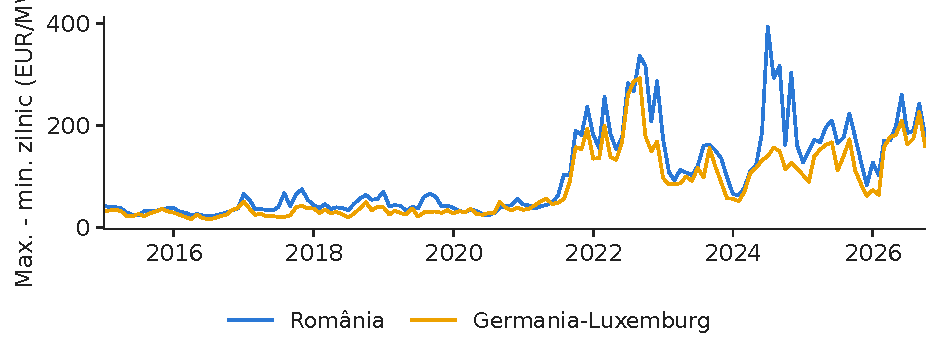
\includegraphics[width=\textwidth,height=0.266\textheight,keepaspectratio]{charts/ro/spread_monthly.pdf}\end{center}\vspace{-3mm}
\chartsource{Sursa: energy-charts.info (Fraunhofer ISE), din datele burselor și ale ENTSO-E. Date: 2 ianuarie 2015 - 31 octombrie 2026, media lunară a diferenței zilnice.}
\vspace{0.5mm}
\begin{itemize}\setlength{\itemsep}{0pt}
  \item România: diferența zilnică medie a fost 47{,}9 EUR/MWh în 2019, 164{,}3 în 2025 și 182{,}8 în 2026 pînă acum.
  \item Luna de vîrf, iulie 2024: 394{,}4 EUR/MWh
    \begin{itemize}\setlength{\itemsep}{0pt}
      \item Producția solară coboară acum prețurile de la prînz.
    \end{itemize}
\end{itemize}
\par\vfill\manager{rentabilitatea unei baterii depinde de diferențele viitoare de preț, nu de nivelul prețului.}\par\vspace{0.5mm}
\par\vfill\noindent{\scriptsize\color{FooterGray}(calcul propriu)}\hfill\qlink{NN\_L10\_spread\_monthly}{Quantlets/L10/NN_L10_spread_monthly}\par\vspace{0.5mm}
\end{frame}


\section{Procese decizionale Markov și ecuația Bellman}

\begin{frame}{Cele cinci elemente ale unui proces decizional Markov}
\footnotesize
\intuition{viitorul depinde de trecut doar prin starea și acțiunea curente.}
\begin{columns}[T,onlytextwidth]
\begin{column}{0.52\textwidth}
\[ \mathcal{M}=(\mathcal{S},\mathcal{A},P,R,\gamma) \]\[ P(s'\mid s,a)=\Pr(s_{t+1}=s'\mid s_t=s,a_t=a) \]\[ G_t=\sum_{k=0}^{T-t-1}\gamma^{k}r_{t+k+1},\quad \pi^{*}=\argmax_{\pi}\E_{\pi}[G_0] \]{\footnotesize\begin{itemize}\setlength{\itemsep}{0pt}
  \item \textbf{\txtwhere}
    \begin{itemize}\setlength{\itemsep}{0pt}
      \item $\mathcal{S},\mathcal{A}$ = stări și acțiuni, $P$ = legea de tranziție, $R(s,a)=\E[r_{t+1}\mid s,a]$
      \item $\gamma\in[0,1]$ = factorul de actualizare, $G_t$ = cîștigul cumulat, $\pi(a\mid s)$ = politica.
    \end{itemize}
\end{itemize}\par}
\end{column}
\begin{column}{0.45\textwidth}
\begin{itemize}\setlength{\itemsep}{3pt}
  \item \textbf{Proprietatea Markov}: starea trebuie să conțină tot ce contează
    \begin{itemize}\setlength{\itemsep}{0pt}
      \item Pentru baterie: ora și energia stocată
      \item Pentru tranzacționare: poziția curentă, deoarece ea determină costul tranzacției următoare.
    \end{itemize}
  \item \textbf{Actualizarea}: $\gamma=1$ pentru episoadele de o zi ale bateriei (24 de pași), $\gamma=0{,}99$ pentru tranzacționare.
  \item \textbf{Orizont finit}: bateria pornește goală în fiecare zi, iar valoarea ei la miezul nopții este zero.
\end{itemize}
\end{column}
\end{columns}
\par\vfill\manager{o variabilă de stare omisă, de exemplu poziția curentă, face agentul instabil.}\par\vspace{0.5mm}
\par\vfill\noindent{\scriptsize\color{FooterGray}(Sutton \& Barto, 2018, ch.\ 3)}\par\vspace{0.5mm}
\end{frame}

\begin{frame}{Funcțiile de valoare măsoară cît de bună este o stare}
\footnotesize
\intuition{$V$ este recompensa viitoare așteptată dintr-o stare; $Q$ este același lucru după o primă acțiune dată.}
\begin{columns}[T,onlytextwidth]
\begin{column}{0.52\textwidth}
\[ V^{\pi}(s)=\E_{\pi}[G_t\mid s_t=s] \]\[ Q^{\pi}(s,a)=\E_{\pi}[G_t\mid s_t=s,a_t=a] \]\[ A^{\pi}(s,a)=Q^{\pi}(s,a)-V^{\pi}(s) \]{\footnotesize\begin{itemize}\setlength{\itemsep}{0pt}
  \item \textbf{\txtwhere}
    \begin{itemize}\setlength{\itemsep}{0pt}
      \item $A^{\pi}$ = avantajul acțiunii $a$ față de acțiunea medie a politicii
      \item Politica optimă este lacomă în raport cu $Q^{*}$: $\pi^{*}(s)=\argmax_a Q^{*}(s,a)$.
    \end{itemize}
\end{itemize}\par}
\end{column}
\begin{column}{0.45\textwidth}
\begin{itemize}\setlength{\itemsep}{3pt}
  \item \textbf{Metodele bazate pe valoare} (Q-learning, DQN) estimează $Q^{*}$ și acționează lacom.
  \item \textbf{Metodele bazate pe politică} (REINFORCE, PPO) parametrizează direct $\pi_{\btheta}$ și folosesc $V$ doar ca reper.
  \item \textbf{Exemplul bateriei}: $V_h(s)$ = numărul de euro care mai pot fi cîștigați azi de la ora $h$, cu $s$ MWh stocați.
\end{itemize}
\end{column}
\end{columns}
\par\vfill\manager{$V$ evaluează un activ (o baterie încărcată, o poziție deschisă)
    \begin{itemize}\setlength{\itemsep}{0pt}
      \item $Q$ compară decizii.
    \end{itemize}}\par\vspace{0.5mm}
\par\vfill\noindent{\scriptsize\color{FooterGray}(Sutton \& Barto, 2018, ch.\ 3--4)}\par\vspace{0.5mm}
\end{frame}

\begin{frame}{Ecuația Bellman: descompunerea recursivă a funcției de valoare}
\footnotesize
\intuition{valoarea optimă acum = cea mai bună recompensă imediată + valoarea optimă actualizată a stării în care ajungeți.}
\begin{columns}[T,onlytextwidth]
\begin{column}{0.53\textwidth}
\[ V^{*}(s)=\max_{a}\Big\{R(s,a)+\gamma\sum_{s'}P(s'\mid s,a)\,V^{*}(s')\Big\} \]\[ Q^{*}(s,a)=R(s,a)+\gamma\,\E_{s'}\big[\max_{a'}Q^{*}(s',a')\big] \]{\footnotesize\begin{itemize}\setlength{\itemsep}{0pt}
  \item \textbf{\txtwhere}
    \begin{itemize}\setlength{\itemsep}{0pt}
      \item Pentru $\gamma<1$ membrul drept este o contracție, deci iterarea valorii $V_{k+1}=\mathcal{T}V_k$ converge la punctul fix unic $V^{*}$
      \item Pe un orizont finit, o singură trecere înapoi dă soluția exactă.
    \end{itemize}
\end{itemize}\par}
\end{column}
\begin{column}{0.44\textwidth}
\begin{itemize}\setlength{\itemsep}{3pt}
  \item \textbf{Principiul optimalității} (Bellman, 1957): un plan optim rămîne optim din orice stare intermediară.
  \item \textbf{Blestemul dimensionalității}: tabelul are $|\mathcal{S}|\times|\mathcal{A}|$ celule
    \begin{itemize}\setlength{\itemsep}{0pt}
      \item Rețelele neuronale înlocuiesc tabelul cînd starea este mare.
    \end{itemize}
  \item \textbf{Modelul este necesar}: DP folosește $P$ și $R$
    \begin{itemize}\setlength{\itemsep}{0pt}
      \item Q-learning și DQN înlocuiesc speranța matematică prin eșantioane.
    \end{itemize}
\end{itemize}
\end{column}
\end{columns}
\par\vfill\manager{fiecare algoritm RL din acest curs este o metodă aproximativă de rezolvare a acestei ecuații.}\par\vspace{0.5mm}
\par\vfill\noindent{\scriptsize\color{FooterGray}(Bellman, 1957; Sutton \& Barto, 2018, ch.\ 4)}\par\vspace{0.5mm}
\end{frame}

\begin{frame}{Bateria ca proces decizional Markov}
\footnotesize
\intuition{starea = (ora, energia stocată); acțiunea = încărcare, inactivitate sau descărcare; recompensa = fluxul de numerar al orei.}
\begin{columns}[T,onlytextwidth]
\begin{column}{0.5\textwidth}
\[ s_{h+1}=s_h-a_h,\quad s_h\in\{0,1,2\}\ \text{MWh},\quad a_h\in\{-1,0,+1\} \]\[ r_h(a_h)=\begin{cases}\eta_d\,p_h & a_h=+1\ (vînzare)\\ -p_h/\eta_c & a_h=-1\ (cumpărare)\\ 0 & a_h=0\end{cases} \]{\footnotesize\begin{itemize}\setlength{\itemsep}{0pt}
  \item \textbf{\txtwhere}
    \begin{itemize}\setlength{\itemsep}{0pt}
      \item $p_h$ = prețul orei $h$ (EUR/MWh), $\eta_c=\eta_d=\sqrt{0{,}85}$ (85\,\% pe ciclu)
      \item 2 MWh, 1 MWh mutat pe oră, goală la 0:00.
    \end{itemize}
\end{itemize}\par}
\end{column}
\begin{column}{0.47\textwidth}
\begin{itemize}\setlength{\itemsep}{3pt}
  \item \textbf{Restricție}: nu se încarcă atunci cînd este plină și nu se descarcă atunci cînd este goală (mascarea acțiunilor).
  \item \textbf{Date}: 4\,292 de zile de livrare din România cu 24 de ore complete, 2 ianuarie 2015 -- 31 octombrie 2026
    \begin{itemize}\setlength{\itemsep}{0pt}
      \item Din oct.\ 2025, ora este media a patru prețuri de 15 minute.
    \end{itemize}
  \item \textbf{Simplificări}: bateria nu influențează prețul
    \begin{itemize}\setlength{\itemsep}{0pt}
      \item Fără cost de degradare, tarife de rețea sau servicii de sistem.
    \end{itemize}
\end{itemize}
\end{column}
\end{columns}
\par\vfill\manager{energia stocată este cea care face decizia secvențială.}\par\vspace{0.5mm}
\par\vfill\noindent{\scriptsize\color{FooterGray}(calcul propriu)}\hfill\tryit{notebook \S2}\par\vspace{0.5mm}
\end{frame}

\begin{frame}{Programarea dinamică rezolvă exact ziua bateriei}
\footnotesize
\intuition{se pornește înapoi de la miezul nopții: la fiecare oră se păstrează cea mai bună acțiune pentru fiecare nivel de energie stocată.}
\begin{columns}[T,onlytextwidth]
\begin{column}{0.53\textwidth}
\[ V_{24}(s)=0 \]\[ V_h(s)=\max_{a:\,0\le s-a\le 2}\big\{r_h(a)+V_{h+1}(s-a)\big\},\quad h=23,\dots,0 \]{\footnotesize\begin{itemize}\setlength{\itemsep}{0pt}
  \item \textbf{\txtwhere}
    \begin{itemize}\setlength{\itemsep}{0pt}
      \item $V_h(s)$ = fluxul de numerar maxim de la ora $h$ la miezul nopții, cu $s$ MWh stocați
      \item Venitul zilei este $V_0(0)$
      \item Argmax în fiecare $(h,s)$ dă acțiunea optimă.
    \end{itemize}
\end{itemize}\par}
\end{column}
\begin{column}{0.44\textwidth}
\begin{itemize}\setlength{\itemsep}{3pt}
  \item \textbf{Cost}: $24\times3\times3$ evaluări pe zi
    \begin{itemize}\setlength{\itemsep}{0pt}
      \item Toate cele 4\,292 de zile în cîteva milisecunde, vectorizat pe zile.
    \end{itemize}
  \item \textbf{Previziune perfectă}: DP folosește cele 24 de prețuri ale zilei înainte ca ele să fie cunoscute, deci venitul său este o \textbf{limită superioară} pentru orice strategie reală.
  \item \textbf{Reperul naiv}: se calculează planul optim de ieri și se aplică azi.
\end{itemize}
\end{column}
\end{columns}
\par\vfill\manager{DP dă plafonul față de care se evaluează orice agent care învață (rata de captare = venit / venitul cu previziune perfectă).}\par\vspace{0.5mm}
\par\vfill\noindent{\scriptsize\color{FooterGray}(Bellman, 1957)}\hfill\tryit{notebook \S2}\par\vspace{0.5mm}
\end{frame}

\begin{frame}{Programul optim al bateriei pentru o zi}
\small
\intuition{în ziua cu cea mai mare diferență de preț din 2026, DP încarcă în orele cele mai ieftine și descarcă în cele mai scumpe.}
\begin{center}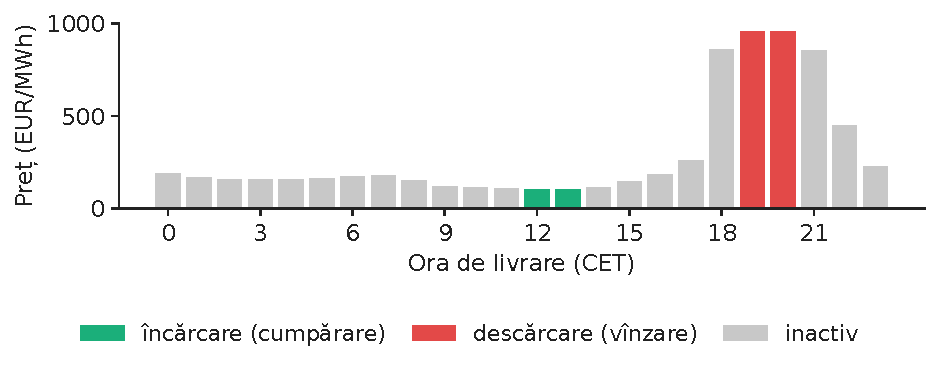
\includegraphics[width=\textwidth,height=0.417\textheight,keepaspectratio]{charts/ro/dp_day.pdf}\end{center}\vspace{-3mm}
\chartsource{Sursa: energy-charts.info (Fraunhofer ISE), din datele burselor și ale ENTSO-E. Date: România, 30 iunie 2026, prețuri orare pentru ziua următoare.}
\vspace{0.5mm}
\begin{itemize}\setlength{\itemsep}{0pt}
  \item 30 iunie 2026: prețuri de la 100{,}65 (ora 13) la 954{,}59 EUR/MWh (ora 20)
    \begin{itemize}\setlength{\itemsep}{0pt}
      \item 2 ore de încărcare și 2 ore de descărcare.
    \end{itemize}
  \item Venitul zilei pentru o baterie de 2 MWh: 1\,541 EUR.
\end{itemize}
\par\vfill\noindent{\scriptsize\color{FooterGray}(calcul propriu)}\hfill\qlink{NN\_L10\_dp\_day}{Quantlets/L10/NN_L10_dp_day}\par\vspace{0.5mm}
\end{frame}

\begin{frame}{Funcția de valoare evaluează energia stocată oră de oră}
\small
\intuition{$V_h(2)-V_h(0)$ arată cît valorează doi MWh stocați la ora $h$: mult înaintea vîrfului de seară, zero după el.}
\begin{center}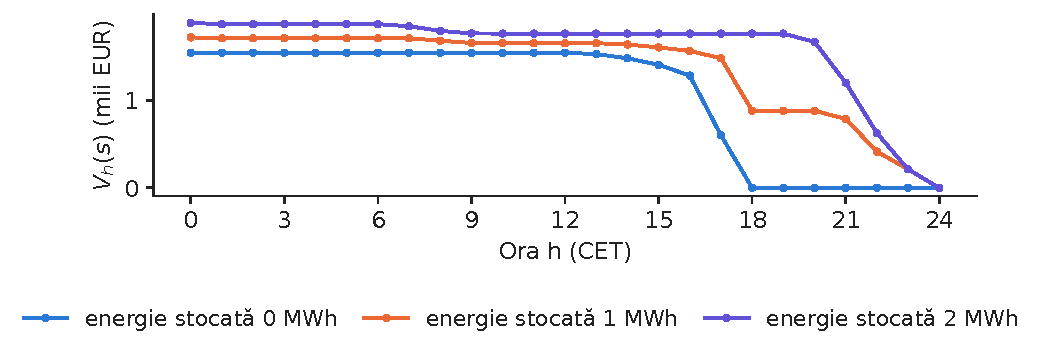
\includegraphics[width=\textwidth,height=0.400\textheight,keepaspectratio]{charts/ro/dp_value.pdf}\end{center}\vspace{-3mm}
\chartsource{Sursa: energy-charts.info (Fraunhofer ISE), din datele burselor și ale ENTSO-E. Date: România, 30 iunie 2026; calcul propriu (inducție înapoi).}
\vspace{0.5mm}
\begin{itemize}\setlength{\itemsep}{0pt}
  \item La ora 12:00, pe 30 iunie 2026: $V_{12}(0)$ = 1\,541 EUR, $V_{12}(2)$ = 1\,760 EUR, deci un MWh stocat valorează 109{,}38 EUR, prețul-umbră al energiei din baterie.
  \item Un $Q$ bine învățat trebuie să reproducă această formă fără să vadă prețurile zilei.
\end{itemize}
\par\vfill\noindent{\scriptsize\color{FooterGray}(calcul propriu)}\hfill\qlink{NN\_L10\_dp\_value}{Quantlets/L10/NN_L10_dp_value}\par\vspace{0.5mm}
\end{frame}

\begin{frame}{Venitul unei baterii de 2 MWh în condiții de previziune perfectă}
\small
\intuition{venitul DP este o limită superioară; el urmează diferențele de preț, nu nivelul prețului.}
\begin{center}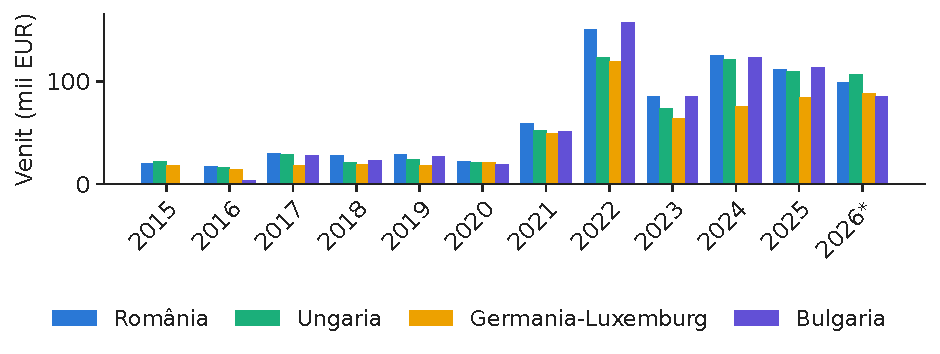
\includegraphics[width=\textwidth,height=0.350\textheight,keepaspectratio]{charts/ro/dp_revenue_year.pdf}\end{center}\vspace{-3mm}
\chartsource{Sursa: energy-charts.info (Fraunhofer ISE), din datele burselor și ale ENTSO-E. Date: 2015-2026 (*2026: ianuarie-octombrie); zile cu 24 de ore complete.}
\vspace{0.5mm}
\begin{itemize}\setlength{\itemsep}{0pt}
  \item România: 28{,}4 mii EUR în 2019, 150{,}2 în 2022, 111{,}2 în 2025, 98{,}5 în 2026, pe 302 de zile.
  \item 2025: Ungaria 109{,}9, Bulgaria 112{,}9, Germania-Luxemburg 84{,}3 mii EUR.
\end{itemize}
\par\vfill\manager{investitorii dimensionează stocarea pe baza acestor cifre
    \begin{itemize}\setlength{\itemsep}{0pt}
      \item Un operator real obține doar o parte, cum se măsoară în secțiunea următoare.
    \end{itemize}}\par\vspace{0.5mm}
\par\vfill\noindent{\scriptsize\color{FooterGray}(calcul propriu)}\hfill\qlink{NN\_L10\_dp\_revenue\_year}{Quantlets/L10/NN_L10_dp_revenue_year}\par\vspace{0.5mm}
\end{frame}


\section{Învățarea bazată pe valoare: Q-learning și DQN}

\begin{frame}{Q-learning: $Q^{*}$ învățat din eșantioane, fără model}
\footnotesize
\intuition{$Q(s,a)$ se deplasează spre recompensă plus cea mai bună valoare a stării următoare; diferența este eroarea de diferență temporală (TD).}
\begin{columns}[T,onlytextwidth]
\begin{column}{0.56\textwidth}
\[ Q(s_t,a_t)\leftarrow Q(s_t,a_t)+\alpha\,\underbrace{\big[r_{t+1}+\gamma\max_{a'}Q(s_{t+1},a')-Q(s_t,a_t)\big]}_{\text{TD error }\delta_t} \]{\footnotesize\begin{itemize}\setlength{\itemsep}{0pt}
  \item \textbf{\txtwhere}
    \begin{itemize}\setlength{\itemsep}{0pt}
      \item $\alpha$ = pasul de învățare (0{,}05 aici)
      \item Ținta folosește acțiunea lacomă din $s_{t+1}$, indiferent ce face agentul în continuare, deci Q-learning este \textbf{off-policy}.
    \end{itemize}
\end{itemize}\par}
\end{column}
\begin{column}{0.41\textwidth}
\begin{itemize}\setlength{\itemsep}{3pt}
  \item \textbf{Convergența} (Watkins \& Dayan, 1992): fiecare pereche $(s,a)$ vizitată de o infinitate de ori, $\sum\alpha_t=\infty$, $\sum\alpha_t^2<\infty$ (Anexa A).
  \item \textbf{Explorarea}: $\varepsilon$-lacom
    \begin{itemize}\setlength{\itemsep}{0pt}
      \item Acțiune aleatoare cu probabilitatea $\varepsilon$, redusă de la 1 la 0{,}05.
    \end{itemize}
  \item \textbf{Riscul exploatării}: fără explorare, o estimare proastă de la început nu mai este corectată.
\end{itemize}
\end{column}
\end{columns}
\par\vfill\manager{eroarea TD este un semnal de învățare disponibil după fiecare oră, nu doar la sfîrșitul zilei.}\par\vspace{0.5mm}
\par\vfill\noindent{\scriptsize\color{FooterGray}(Watkins \& Dayan, 1992)}\hfill\tryit{notebook \S3}\par\vspace{0.5mm}
\end{frame}

\begin{frame}{Definirea stării: informația disponibilă agentului}
\footnotesize
\intuition{operatorul planifică înainte să cunoască prețurile pentru ziua următoare; agentul ține cont de cît de ieftină a fost fiecare oră ieri.}
\begin{columns}[T,onlytextwidth]
\begin{column}{0.55\textwidth}
\[ s_h=\big(h,\ \text{stored}_h,\ q_{h}\big),\quad q_h=\Big\lfloor\tfrac{\mathrm{rank}(p^{\,\text{ieri}}_h)}{6}\Big\rfloor\in\{0,1,2,3\} \]{\footnotesize\begin{itemize}\setlength{\itemsep}{0pt}
  \item \textbf{\txtwhere}
    \begin{itemize}\setlength{\itemsep}{0pt}
      \item Rangul orei $h$ între cele 24 de prețuri de ieri, deci $q_h=0$ = una dintre cele mai ieftine șase ore de ieri
      \item Tabelul are $24\times4\times3$ stări $\times$ 3 acțiuni.
    \end{itemize}
\end{itemize}\par}
\end{column}
\begin{column}{0.42\textwidth}
\begin{itemize}\setlength{\itemsep}{3pt}
  \item \textbf{Antrenare}: 1\,746 de zile din 2019--2023, 40 de treceri
    \begin{itemize}\setlength{\itemsep}{0pt}
      \item Se păstrează epoca cu cel mai mare venit de validare în 2024.
    \end{itemize}
  \item \textbf{Test}: 638 de zile, 1 ianuarie 2025 -- 24 octombrie 2026, folosite o singură dată.
  \item \textbf{Scara recompensei}: EUR/100, $\gamma=1$ în cursul zilei.
\end{itemize}
\end{column}
\end{columns}
\par\vfill\manager{o stare care include prețurile de azi ar da un test retrospectiv perfect, dar inutil.}\par\vspace{0.5mm}
\par\vfill\noindent{\scriptsize\color{FooterGray}(calcul propriu)}\hfill\tryit{notebook \S3}\par\vspace{0.5mm}
\end{frame}

\begin{frame}{Politica învățată prin Q-learning tabelar}
\small
\intuition{cu 1 MWh stocat, agentul încarcă în orele care au fost ieftine ieri și vinde seara.}
\begin{center}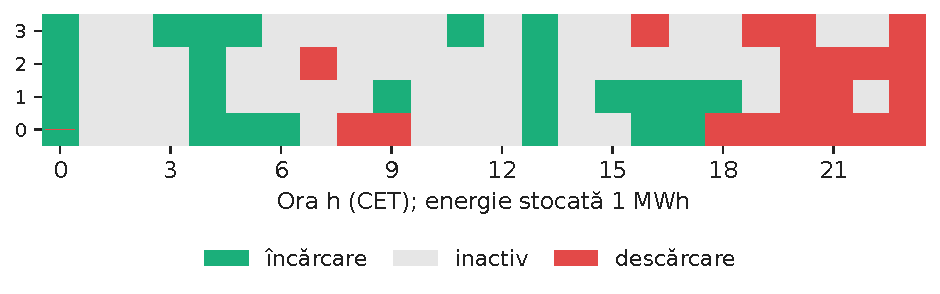
\includegraphics[width=\textwidth,height=0.460\textheight,keepaspectratio]{charts/ro/q_policy.pdf}\end{center}\vspace{-3mm}
\chartsource{Sursa: energy-charts.info (Fraunhofer ISE), din datele burselor și ale ENTSO-E. Date: rînduri = quartila prețului orei respective în ziua precedentă; valoarea inițială 20261108.}
\vspace{0.5mm}
\begin{itemize}\setlength{\itemsep}{0pt}
  \item O politică ușor de citit: tabelul poate fi tipărit și verificat oră cu oră (288 de stări).
  \item Ora din zi domină
    \begin{itemize}\setlength{\itemsep}{0pt}
      \item Clasamentul de ieri mută momentul încărcării.
    \end{itemize}
\end{itemize}
\par\vfill\noindent{\scriptsize\color{FooterGray}(calcul propriu)}\hfill\qlink{NN\_L10\_q\_policy}{Quantlets/L10/NN_L10_q_policy}\par\vspace{0.5mm}
\end{frame}

\begin{frame}{Rețeaua Q profundă: aproximarea tabelului Q printr-o rețea neuronală}
\footnotesize
\intuition{tabelul este înlocuit de o rețea $Q_{\btheta}(s,a)$, ajustată prin regresie pe ținta TD.}
\begin{columns}[T,onlytextwidth]
\begin{column}{0.56\textwidth}
\[ y=r+\gamma\,Q_{\btheta^{-}}\big(s',\argmax_{a'}Q_{\btheta}(s',a')\big) \]\[ \loss(\btheta)=\E_{(s,a,r,s')\sim\mathcal{D}}\big[\ell_{\text{Huber}}\big(y-Q_{\btheta}(s,a)\big)\big] \]{\footnotesize\begin{itemize}\setlength{\itemsep}{0pt}
  \item \textbf{\txtwhere}
    \begin{itemize}\setlength{\itemsep}{0pt}
      \item $\mathcal{D}$ = memoria de reluare (ultimele patru epoci)
      \item $\btheta^{-}$ = rețeaua-țintă, o copie lentă $\btheta^{-}\leftarrow(1-\tau)\btheta^{-}+\tau\btheta$, $\tau=0{,}005$
      \item DQN dublu: rețeaua online alege $a'$, rețeaua-țintă o evaluează.
    \end{itemize}
\end{itemize}\par}
\end{column}
\begin{column}{0.41\textwidth}
\begin{itemize}\setlength{\itemsep}{3pt}
  \item \textbf{Reluarea} elimină corelația dintre orele consecutive (Mnih et al., 2015).
  \item \textbf{DQN dublu} elimină deplasarea în sus a lui $\max_{a'}$ aplicat unor estimări zgomotoase (van Hasselt et al., 2016).
  \item \textbf{Rețeaua noastră}: 82 de intrări (cele 24 de prețuri standardizate de ieri și din aceeași zi a săptămînii trecute, ziua săptămînii, ora, energia stocată), două straturi de cîte 128 de unități liniare rectificate (ReLU), 3 ieșiri.
\end{itemize}
\end{column}
\end{columns}
\par\vfill\manager{aproximarea funcției, autoreferința țintei și datele off-policy pot produce divergență
    \begin{itemize}\setlength{\itemsep}{0pt}
      \item Reluarea și rețeaua-țintă mențin stabilitatea.
    \end{itemize}}\par\vspace{0.5mm}
\par\vfill\noindent{\scriptsize\color{FooterGray}(Mnih et al., 2015; van Hasselt, Guez \& Silver, 2016)}\hfill\tryit{notebook \S4}\par\vspace{0.5mm}
\end{frame}

\begin{frame}{Curbele de învățare: venitul de validare pe epoci}
\small
\intuition{ambii agenți progresează repede, dar rămîn sub planul de ieri; epoca păstrată este cea mai bună pe 2024, niciodată pe anii de test.}
\begin{center}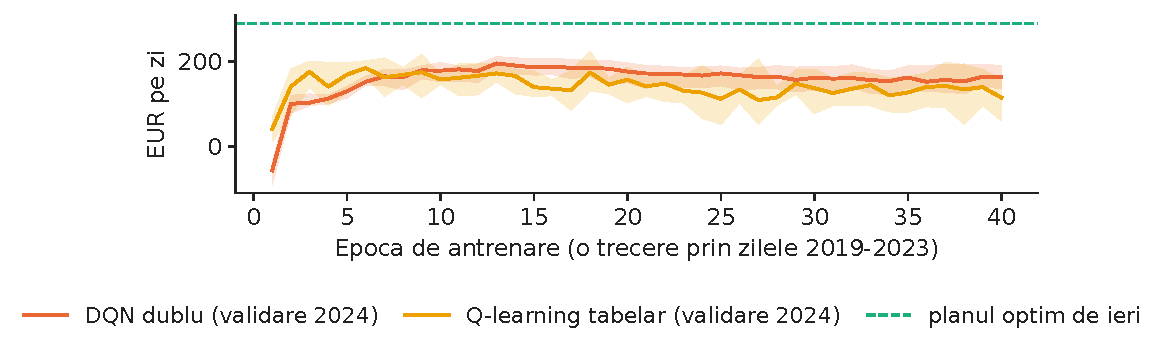
\includegraphics[width=\textwidth,height=0.449\textheight,keepaspectratio]{charts/ro/battery_learning.pdf}\end{center}\vspace{-3mm}
\chartsource{Sursa: energy-charts.info (Fraunhofer ISE), din datele burselor și ale ENTSO-E. Date: anul de validare 2024; banda = intervalul celor 5 valori inițiale.}
\vspace{0.5mm}
\begin{itemize}\setlength{\itemsep}{0pt}
  \item Cel mai bun venit de validare pe zi, media a 5 valori inițiale: DQN 200 EUR, Q-learning 211 EUR, planul de ieri 289 EUR.
\end{itemize}
\par\vfill\noindent{\scriptsize\color{FooterGray}(calcul propriu)}\hfill\qlink{NN\_L10\_battery\_learning}{Quantlets/L10/NN_L10_battery_learning}\par\vspace{0.5mm}
\end{frame}

\begin{frame}{Ponderea venitului cu previziune perfectă obținută în anii de test}
\small
\intuition{venitul cumulat de la 1 ianuarie 2025 la 24 octombrie 2026; distanța față de linia de sus este valoarea informației perfecte.}
\begin{center}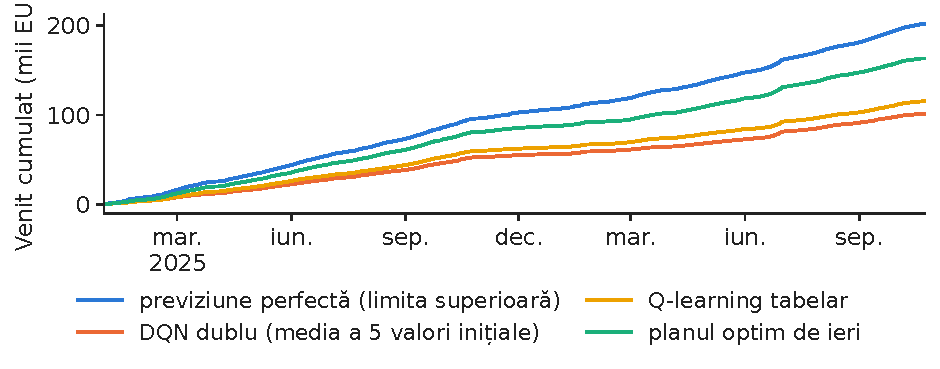
\includegraphics[width=\textwidth,height=0.387\textheight,keepaspectratio]{charts/ro/battery_test_cum.pdf}\end{center}\vspace{-3mm}
\chartsource{Sursa: energy-charts.info (Fraunhofer ISE), din datele burselor și ale ENTSO-E. Date: 1 ianuarie 2025 - 24 octombrie 2026 (test); antrenare 2019-2023, validare 2024.}
\vspace{0.5mm}
\begin{itemize}\setlength{\itemsep}{0pt}
  \item Previziune perfectă 202{,}1
    \begin{itemize}\setlength{\itemsep}{0pt}
      \item DQN 101{,}3
      \item Q-learning 115{,}2
      \item Planul de ieri 163{,}1 mii EUR.
    \end{itemize}
\end{itemize}
\par\vfill\noindent{\scriptsize\color{FooterGray}(calcul propriu)}\hfill\qlink{NN\_L10\_battery\_test\_cum}{Quantlets/L10/NN_L10_battery_test_cum}\par\vspace{0.5mm}
\end{frame}

\begin{frame}{Rezultatele bateriei pe anii de test, cinci valori inițiale}
\small
{\small\renewcommand{\arraystretch}{1.05}\setlength{\tabcolsep}{4pt}
\begin{tabular}{@{}p{0.36\textwidth}rrr@{}}\toprule
Strategia & Venit (mii EUR) & Captare (\%) & Interval (\%) \\ \midrule
Previziune perfectă (DP, limita superioară) & 202{,}1 & 100 & -- \\
DQN dublu & 101{,}3 & 50{,}1 & 43{,}9 -- 58{,}5 \\
Q-learning tabelar & 115{,}2 & 57{,}0 & 50{,}2 -- 61{,}9 \\
Planul optim de ieri (naiv) & 163{,}1 & 80{,}7 & -- \\
\bottomrule\end{tabular}}\vspace{2mm}\begin{itemize}\setlength{\itemsep}{2pt}
  \item \textbf{DQN față de planul naiv}: statistica Diebold-Mariano (DM) pe diferențele zilnice, varianță Newey-West (7 decalaje): $t$ = \ensuremath{-}18{,}99, $p$ = 0{,}000
    \begin{itemize}\setlength{\itemsep}{0pt}
      \item Diferența medie \ensuremath{-}96{,}8 EUR pe zi.
    \end{itemize}
  \item DQN bate planul naiv pentru 0 din 5 valori inițiale, Q-learning pentru 0 din 5: regula simplă cîștigă, pentru că optimizează pe toate cele 24 de prețuri de ieri.
\end{itemize}
\par\vfill\manager{raportați rata de captare cu intervalul pe valori inițiale și un test față de planul naiv, niciodată doar cea mai bună rulare.}\par\vspace{0.5mm}
\par\vfill\noindent{\scriptsize\color{FooterGray}(Diebold \& Mariano, 1995; calcul propriu)}\hfill\tryit{notebook \S4}\par\vspace{0.5mm}
\end{frame}


\section{Gradienți de politică și PPO: tranzacționarea indicelui S\&P 500}

\begin{frame}{Metodele de gradient al politicii}
\footnotesize
\intuition{politica se parametrizează direct și se urcă pe gradientul cîștigului așteptat.}
\begin{columns}[T,onlytextwidth]
\begin{column}{0.55\textwidth}
\[ \nabla_{\btheta}J(\btheta)=\E_{\pi_{\btheta}}\Big[\sum_{t}\nabla_{\btheta}\log\pi_{\btheta}(a_t\mid s_t)\,\big(G_t-b(s_t)\big)\Big] \]{\footnotesize\begin{itemize}\setlength{\itemsep}{0pt}
  \item \textbf{\txtwhere}
    \begin{itemize}\setlength{\itemsep}{0pt}
      \item $J(\btheta)=\E_{\pi_{\btheta}}[G_0]$
      \item $\nabla\log\pi$ = funcția scor
      \item $b(s_t)$ = reperul, orice funcție de stare, care lasă gradientul nedeplasat și îi reduce varianța
      \item $b=V_{\boldsymbol{\phi}}(s_t)$ dă o metodă actor-critic.
    \end{itemize}
\end{itemize}\par}
\end{column}
\begin{column}{0.42\textwidth}
\begin{itemize}\setlength{\itemsep}{3pt}
  \item \textbf{REINFORCE} (Williams, 1992): $G_t$ estimat Monte Carlo
    \begin{itemize}\setlength{\itemsep}{0pt}
      \item Nedeplasat, varianță mare.
    \end{itemize}
  \item \textbf{Teorema gradientului politicii} (Sutton et al., 2000): gradientul nu cere derivata legii de tranziție, deci piața poate rămîne o cutie neagră.
  \item \textbf{Politicile stocastice} explorează singure și tratează acțiuni continue.
\end{itemize}
\end{column}
\end{columns}
\par\vfill\manager{trucul log-verosimilității este același folosit la antrenarea clasificatorilor, ponderat cu cît de bun a fost rezultatul.}\par\vspace{0.5mm}
\par\vfill\noindent{\scriptsize\color{FooterGray}(Williams, 1992; Sutton et al., 2000)}\par\vspace{0.5mm}
\end{frame}

\begin{frame}{Actor-critic și estimarea avantajului}
\footnotesize
\intuition{un critic $V_{\boldsymbol{\phi}}$ prognozează cîștigul, iar actorul învață din surpriza $\hat A_t$.}
\begin{columns}[T,onlytextwidth]
\begin{column}{0.56\textwidth}
\[ \delta_t=r_{t+1}+\gamma V_{\boldsymbol{\phi}}(s_{t+1})-V_{\boldsymbol{\phi}}(s_t),\qquad \hat A_t=\sum_{l\ge0}(\gamma\lambda)^{l}\,\delta_{t+l} \]\[ \loss_V(\boldsymbol{\phi})=\E\big[(\hat A_t+V_{\boldsymbol{\phi}}^{\text{old}}(s_t)-V_{\boldsymbol{\phi}}(s_t))^2\big] \]{\footnotesize\begin{itemize}\setlength{\itemsep}{0pt}
  \item \textbf{\txtwhere}
    \begin{itemize}\setlength{\itemsep}{0pt}
      \item Estimarea generalizată a avantajului (GAE): $\lambda=0$ dă avantajul TD de un pas (varianță mică, deplasat), $\lambda=1$ avantajul Monte Carlo
      \item Folosim $\gamma=0{,}99$, $\lambda=0{,}95$.
    \end{itemize}
\end{itemize}\par}
\end{column}
\begin{column}{0.41\textwidth}
\begin{itemize}\setlength{\itemsep}{3pt}
  \item \textbf{Trunchi comun}: actorul și criticul împart două straturi de cîte 64 de unități tanh
    \begin{itemize}\setlength{\itemsep}{0pt}
      \item Ieșiri: 2 logiți pentru acțiuni și o valoare.
    \end{itemize}
  \item \textbf{Normalizarea avantajului} în fiecare lot păstrează pasul comparabil între regimuri de piață.
  \item \textbf{Bonusul de entropie} 0{,}01 împiedică politica să devină deterministă prea devreme.
\end{itemize}
\end{column}
\end{columns}
\par\vfill\manager{criticul este o prognoză a recompensei viitoare
    \begin{itemize}\setlength{\itemsep}{0pt}
      \item Un critic slab dă avantaje zgomotoase și o învățare lentă.
    \end{itemize}}\par\vspace{0.5mm}
\par\vfill\noindent{\scriptsize\color{FooterGray}(Schulman et al., 2016)}\par\vspace{0.5mm}
\end{frame}

\begin{frame}{PPO: actualizarea plafonată a politicii}
\small
\intuition{obiectivul plafonat elimină stimulentul de a muta raportul probabilităților în afara intervalului $[1-\epsilon,1+\epsilon]$.}
\vspace{-1mm}\[ \loss^{\text{CLIP}}(\btheta)=\E_t\big[\min\big(\rho_t\hat A_t,\ \mathrm{clip}(\rho_t,1-\epsilon,1+\epsilon)\hat A_t\big)\big],\quad \rho_t=\frac{\pi_{\btheta}(a_t\mid s_t)}{\pi_{\btheta_{\text{old}}}(a_t\mid s_t)} \]\vspace{-2mm}
\begin{center}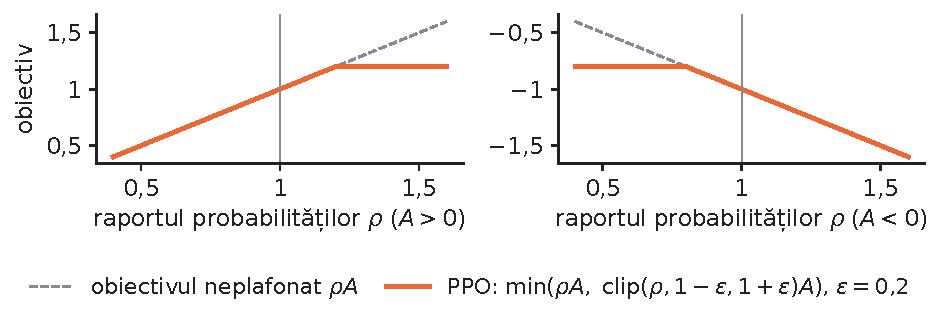
\includegraphics[width=\textwidth,height=0.322\textheight,keepaspectratio]{charts/ro/ppo_clip.pdf}\end{center}\vspace{-3mm}
\chartsource{Sursa: Schulman et al. (2017), obiectivul surogat plafonat. Date: funcție analitică, fără date.}
\vspace{0.5mm}
\begin{itemize}\setlength{\itemsep}{0pt}
  \item \simlabel\ Funcție analitică, fără date
    \begin{itemize}\setlength{\itemsep}{0pt}
      \item $\epsilon=0{,}2$
      \item Un înlocuitor ieftin al regiunii de încredere bazate pe divergența Kullback-Leibler (KL) din optimizarea politicii în regiune de încredere (TRPO).
    \end{itemize}
\end{itemize}
\par\vfill\noindent{\scriptsize\color{FooterGray}(Schulman et al., 2017)}\hfill\qlink{NN\_L10\_ppo\_clip}{Quantlets/L10/NN_L10_ppo_clip}\par\vspace{0.5mm}
\end{frame}

\begin{frame}{Tranzacționarea ca MDP: în afara pieței sau long pe S\&P 500}
\footnotesize
\intuition{în fiecare seară agentul alege poziția de mîine; cîștigă randamentul zilei următoare și plătește un cost cînd își schimbă poziția.}
\begin{columns}[T,onlytextwidth]
\begin{column}{0.53\textwidth}
\[ r_{t+1}=a_t\,\ln\frac{P_{t+1}}{P_t}-c\,|a_t-a_{t-1}|,\qquad a_t\in\{0,1\},\ c=5\ \text{bp} \]{\footnotesize\begin{itemize}\setlength{\itemsep}{0pt}
  \item \textbf{\txtwhere}
    \begin{itemize}\setlength{\itemsep}{0pt}
      \item $s_t$ = 7 variabile standardizate pe 2005--2016 (randamente pe 1, 5, 21, 63 de zile, volatilitatea pe 21 de zile, VIX, distanța față de media de 200 de zile) + $a_{t-1}$.
    \end{itemize}
\end{itemize}\par}
\end{column}
\begin{column}{0.44\textwidth}
\begin{itemize}\setlength{\itemsep}{2pt}
  \item \textbf{Antrenare}: 150 de iterații PPO cu cîte 64 de ferestre aleatoare de 126 de zile din 2005--2016, plafon 0{,}2.
  \item \textbf{Selecție}: iterația cu cel mai bun raport Sharpe în 2017--2019.
  \item \textbf{Test}: 1\,716 de zile de la 2 ianuarie 2020, cinci valori inițiale, față de cumpără și păstrează și media mobilă de 200 de zile.
\end{itemize}
\end{column}
\end{columns}
\par\vfill\manager{includeți costul în recompensă, altfel agentul tranzacționează mult prea des.}\par\vspace{0.5mm}
\par\vfill\noindent{\scriptsize\color{FooterGray}(Moody \& Saffell, 2001; calcul propriu)}\hfill\tryit{notebook \S5}\par\vspace{0.5mm}
\end{frame}

\begin{frame}{Raportul Sharpe la antrenare și validare în timpul antrenării PPO}
\small
\intuition{raportul Sharpe de antrenare crește; cel de validare este zgomotos, iar cea mai bună iterație este păstrată.}
\begin{center}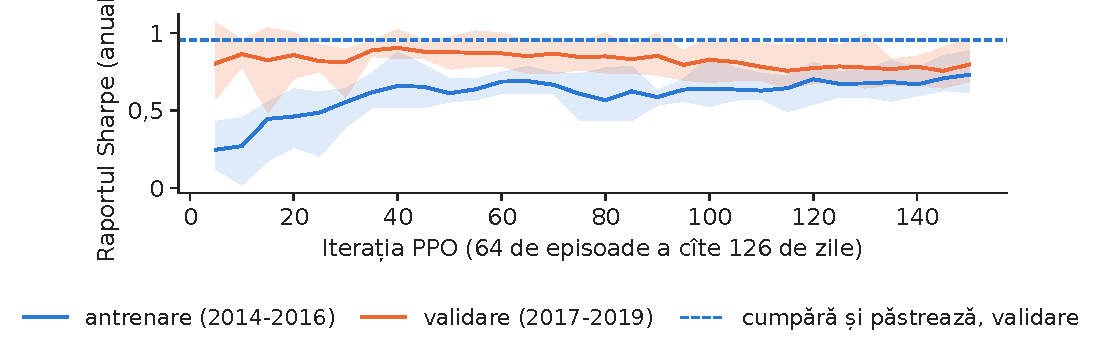
\includegraphics[width=\textwidth,height=0.472\textheight,keepaspectratio]{charts/ro/trading_learning.pdf}\end{center}\vspace{-3mm}
\chartsource{Sursa: Yahoo Finance, cotații zilnice. Date: ferestre de antrenare din 17 octombrie 2005 - 30 decembrie 2016; banda = intervalul celor 5 valori inițiale.}
\vspace{0.5mm}
\begin{itemize}\setlength{\itemsep}{0pt}
  \item Raportul Sharpe al strategiei cumpără și păstrează pe validare (2017--2019): 0{,}95
    \begin{itemize}\setlength{\itemsep}{0pt}
      \item Iterația selectată este în medie 48.
    \end{itemize}
\end{itemize}
\par\vfill\noindent{\scriptsize\color{FooterGray}(calcul propriu)}\hfill\qlink{NN\_L10\_trading\_learning}{Quantlets/L10/NN_L10_trading_learning}\par\vspace{0.5mm}
\end{frame}

\begin{frame}{Perioada de test: agentul PPO față de două reguli simple}
\small
\intuition{valoarea unui USD investit la 2 ianuarie 2020, după un cost de 5 puncte de bază la fiecare schimbare de poziție.}
\begin{center}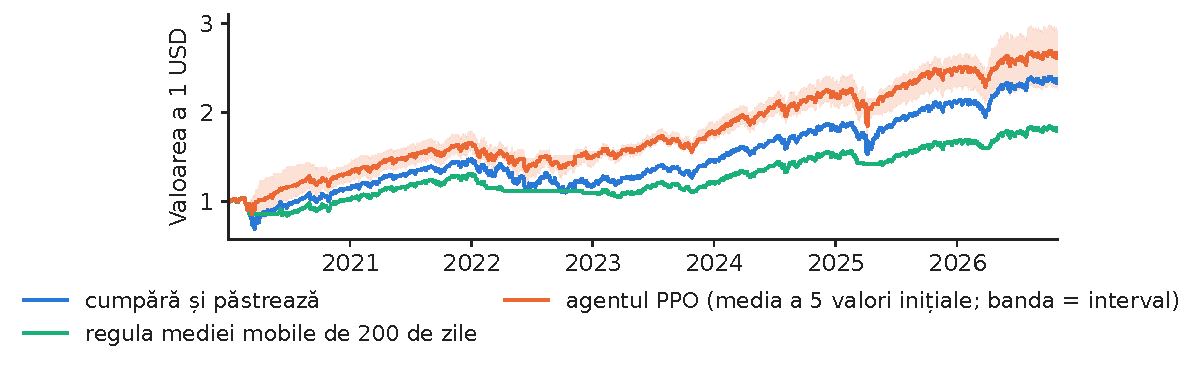
\includegraphics[width=\textwidth,height=0.466\textheight,keepaspectratio]{charts/ro/trading_equity.pdf}\end{center}\vspace{-3mm}
\chartsource{Sursa: Yahoo Finance, cotații zilnice. Date: 2 ianuarie 2020 - 29 octombrie 2026 (test), S\&P 500, cost de 5 pb pe tranzacție.}
\vspace{0.5mm}
\begin{itemize}\setlength{\itemsep}{0pt}
  \item Raportul Sharpe: cumpără și păstrează 0{,}61
    \begin{itemize}\setlength{\itemsep}{0pt}
      \item Regula mediei mobile 0{,}68
      \item PPO 0{,}83 (între 0{,}72 și 0{,}95 pe valori inițiale).
    \end{itemize}
\end{itemize}
\par\vfill\noindent{\scriptsize\color{FooterGray}(calcul propriu)}\hfill\qlink{NN\_L10\_trading\_equity}{Quantlets/L10/NN_L10_trading_equity}\par\vspace{0.5mm}
\end{frame}

\begin{frame}{Rezultatele tranzacționării pe perioada de test}
\small
{\small\renewcommand{\arraystretch}{1.05}\setlength{\tabcolsep}{4pt}
\begin{tabular}{@{}p{0.25\textwidth}rrrrrr@{}}\toprule
Strategia & Rand.\ \%/an & Vol.\ \%/an & Sharpe & Scădere max.\ \% & Investit \% & Tranz. \\ \midrule
Cumpără și păstrează & 13{,}2 & 20{,}2 & 0{,}61 & \ensuremath{-}33{,}9 & 100 & 1 \\
Media mobilă de 200 de zile & 8{,}9 & 12{,}4 & 0{,}68 & \ensuremath{-}20{,}5 & 79 & 41 \\
PPO (media a 5 valori inițiale) & 15{,}1 & 17{,}0 & 0{,}83 & \ensuremath{-}23{,}2 & 82 & 147 \\
\bottomrule\end{tabular}}\vspace{2mm}\begin{itemize}\setlength{\itemsep}{2pt}
  \item \textbf{Incertitudinea}: diferența dintre raportul Sharpe al strategiei PPO mediate pe valori inițiale și cel al strategiei cumpără și păstrează: \ensuremath{+}0{,}26
    \begin{itemize}\setlength{\itemsep}{0pt}
      \item Intervalul de 95\,\% din bootstrap staționar pe blocuri: [\ensuremath{-}0{,}08; 0{,}56] (2\,000 de reeșantionări, bloc mediu de 21 de zile).
    \end{itemize}
  \item PPO bate strategia cumpără și păstrează la raportul Sharpe pentru 5 din 5 valori inițiale.
\end{itemize}
\par\vfill\manager{un interval care conține zero înseamnă că nu există dovezi că agentul aduce valoare, orice ar sugera graficul retrospectiv.}\par\vspace{0.5mm}
\par\vfill\noindent{\scriptsize\color{FooterGray}(Politis \& Romano, 1994; calcul propriu)}\hfill\tryit{notebook \S5}\par\vspace{0.5mm}
\end{frame}

\begin{frame}{Perioadele în care agentul este în afara pieței}
\small
\intuition{expunerea agentului PPO (ponderea valorilor inițiale și a zilelor investite) comparată cu regula mediei mobile.}
\begin{center}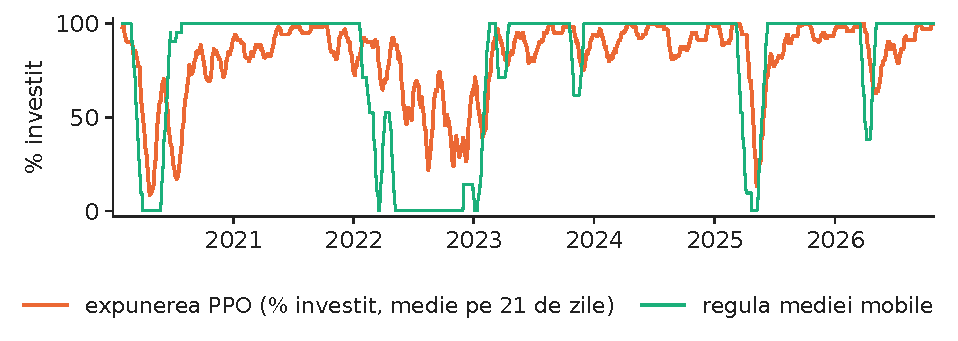
\includegraphics[width=\textwidth,height=0.340\textheight,keepaspectratio]{charts/ro/trading_exposure.pdf}\end{center}\vspace{-3mm}
\chartsource{Sursa: Yahoo Finance, cotații zilnice. Date: 2 ianuarie 2020 - 29 octombrie 2026 (test).}
\vspace{0.5mm}
\begin{itemize}\setlength{\itemsep}{0pt}
  \item Investit: PPO 82\,\% din zilele de test
    \begin{itemize}\setlength{\itemsep}{0pt}
      \item 20 feb.\ -- 30 apr.\ 2020 42\,\% (media mobilă 14\,\%)
      \item 2022 63\,\% (media mobilă 15\,\%).
    \end{itemize}
\end{itemize}
\par\vfill\manager{citiți politica, nu doar profitul: un agent care este pur și simplu mereu investit este o strategie cumpără și păstrează cu risc de model suplimentar.}\par\vspace{0.5mm}
\par\vfill\noindent{\scriptsize\color{FooterGray}(calcul propriu)}\hfill\qlink{NN\_L10\_trading\_exposure}{Quantlets/L10/NN_L10_trading_exposure}\par\vspace{0.5mm}
\end{frame}

\begin{frame}{Limitele testelor retrospective pentru agenții de tranzacționare}
\small
\begin{itemize}\setlength{\itemsep}{4pt}
  \item \textbf{Raport semnal-zgomot redus}: randamentele zilnice ale acțiunilor sînt aproape imprevizibile
    \begin{itemize}\setlength{\itemsep}{0pt}
      \item Agentul învață mai ales zgomotul ferestrelor de antrenare.
    \end{itemize}
  \item \textbf{Nestaționaritatea}: 2005--2016 conține anul 2008
    \begin{itemize}\setlength{\itemsep}{0pt}
      \item 2020--2026 conține prăbușirea din pandemie, șocul inflației și o creștere lungă.
    \end{itemize}
  \item \textbf{Riscul valorii inițiale și al selecției}: cinci valori inițiale dau deja un interval de rapoarte Sharpe
    \begin{itemize}\setlength{\itemsep}{0pt}
      \item Raportarea celei mai bune este supraajustare retrospectivă.
    \end{itemize}
  \item \textbf{Impactul asupra prețului și costurile}: un simulator în care agentul nu influențează prețul ignoră impactul
    \begin{itemize}\setlength{\itemsep}{0pt}
      \item Costurile trebuie incluse în recompensă, nu adăugate ulterior.
    \end{itemize}
  \item \textbf{Unde ajută mai mult RL}: execuția (împărțirea unui ordin mare), crearea de piață, acoperirea riscului, stocarea: probleme cu o stare reală și o recompensă cunoscută.
\end{itemize}
\par\vfill\manager{cereți distribuția pe valori inițiale, ipoteza de cost și un interval bootstrap înainte de a avea încredere într-un rezultat RL de tranzacționare.}\par\vspace{0.5mm}
\par\vfill\noindent{\scriptsize\color{FooterGray}(Hambly, Xu \& Yang, 2023)}\par\vspace{0.5mm}
\end{frame}


\section{Acoperirea neuronală: o politică ce minimizează riscul din coadă}

\begin{frame}{Acoperirea unei opțiuni call vîndute: rezultatul desk-ului}
\footnotesize
\intuition{desk-ul vinde o opțiune call la bani (ATM) pe o lună și tranzacționează zilnic indicele pentru a compensa riscul.}
\begin{columns}[T,onlytextwidth]
\begin{column}{0.56\textwidth}
\[ \mathrm{PL}(\delta)=C_0+\sum_{k=0}^{20}\delta_k\,(S_{k+1}-S_k)-(S_{21}-K)^{+}-c\sum_{k=0}^{21}S_k\,|\delta_k-\delta_{k-1}| \]{\footnotesize\begin{itemize}\setlength{\itemsep}{0pt}
  \item \textbf{\txtwhere}
    \begin{itemize}\setlength{\itemsep}{0pt}
      \item $S_k$ = închiderea S\&P 500 în ziua $k$ a unei traiectorii reale de 21 de zile, $S_0=K=1$
      \item $C_0$ = prima Black-Scholes (VIX din ziua 0, rata 0), $\delta_k$ = unitățile deținute pe $(k,k+1]$, $c$ = 10 pb.
    \end{itemize}
\end{itemize}\par}
\end{column}
\begin{column}{0.41\textwidth}
\begin{itemize}\setlength{\itemsep}{2pt}
  \item \textbf{Traiectorii}: una pentru fiecare zi de început
    \begin{itemize}\setlength{\itemsep}{0pt}
      \item Antrenare 3\,021 (2005--2016), validare 754, test 1\,696 traiectorii din 2020.
    \end{itemize}
  \item \textbf{Test}: prima medie 2{,}38\,\%, plata medie 2{,}53\,\% din indice (VIX mediu 20{,}7).
  \item \textbf{Real, nu simulat}: traiectoriile păstrează salturile și grupările de volatilitate din 2008, 2020 și 2022.
\end{itemize}
\end{column}
\end{columns}
\par\vfill\manager{prima abia acoperă plata medie
    \begin{itemize}\setlength{\itemsep}{0pt}
      \item Departamentul de risc gestionează coada.
    \end{itemize}}\par\vspace{0.5mm}
\par\vfill\noindent{\scriptsize\color{FooterGray}(Buehler et al., 2019)}\hfill\tryit{notebook \S6}\par\vspace{0.5mm}
\end{frame}

\begin{frame}{Delta Black-Scholes și obiectivul acoperirii neuronale}
\footnotesize
\intuition{reperul acoperă sensibilitatea din model; rețeaua minimizează în schimb pierderea așteptată din coadă a pierderii reale, cu tot cu costuri.}
\begin{columns}[T,onlytextwidth]
\begin{column}{0.56\textwidth}
\[ \delta_k^{\text{BS}}=\Phi(d_1),\quad d_1=\frac{\ln(S_k/K)+\tfrac12\sigma_k^{2}\tau_k}{\sigma_k\sqrt{\tau_k}} \]\[ \min_{\btheta,w}\ w+\frac{1}{1-\alpha}\E\big[(-\mathrm{PL}(\delta_{\btheta})-w)^{+}\big]=\min_{\btheta}\mathrm{ES}_{\alpha}\big(-\mathrm{PL}(\delta_{\btheta})\big) \]{\footnotesize\begin{itemize}\setlength{\itemsep}{0pt}
  \item \textbf{\txtwhere}
    \begin{itemize}\setlength{\itemsep}{0pt}
      \item $\sigma_k$ = VIX/100, $\tau_k=(21-k)/252$, $\alpha=0{,}95$
      \item La optim, $w$ este valoarea la risc (VaR)
      \item $\delta_{\btheta}(\ln S_k,\tau_k,\sigma_k,\delta_{k-1})\in[0,1]$: 2 straturi de cîte 32 de unități ReLU, ieșire sigmoidă.
    \end{itemize}
\end{itemize}\par}
\end{column}
\begin{column}{0.41\textwidth}
\begin{itemize}\setlength{\itemsep}{3pt}
  \item \textbf{Optimizarea politicii cu recompensă cunoscută}: rezultatul este diferențiabil în $\btheta$, deci propagăm gradientul înapoi prin toate cele 21 de zile.
  \item \textbf{Acoperirea anterioară ca intrare}: permite rețelei să învețe o bandă fără tranzacții atunci cînd costurile sînt mari.
  \item \textbf{Antrenare}: 600 de pași Adam pe tot setul, cinci valori inițiale.
\end{itemize}
\end{column}
\end{columns}
\par\vfill\manager{obiectivul este chiar măsura de risc raportată de desk.}\par\vspace{0.5mm}
\par\vfill\noindent{\scriptsize\color{FooterGray}(Buehler et al., 2019; Rockafellar \& Uryasev, 2000)}\hfill\tryit{notebook \S6}\par\vspace{0.5mm}
\end{frame}

\begin{frame}{Rezultatul acoperirii pe traiectoriile de test}
\small
\intuition{acoperirea elimină cea mai mare parte a cozii din stînga; acoperirea neuronală reduce și mai mult coada rămasă, cu un volum tranzacționat mai mic.}
\begin{center}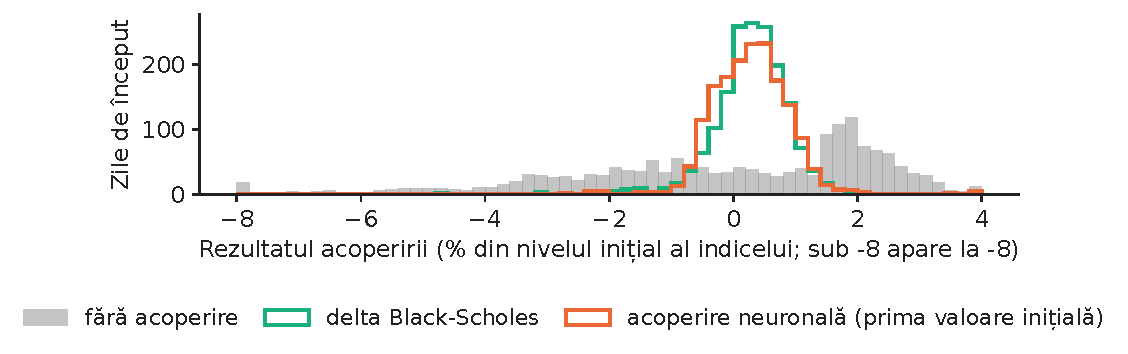
\includegraphics[width=\textwidth,height=0.502\textheight,keepaspectratio]{charts/ro/hedge_pnl.pdf}\end{center}\vspace{-3mm}
\chartsource{Sursa: Yahoo Finance, cotații zilnice. Date: traiectorii de 21 de zile începute 2 ianuarie 2020 - 1 octombrie 2026 (test); S\&P 500 și VIX; cost 10 pb.}
\vspace{0.5mm}
\begin{itemize}\setlength{\itemsep}{0pt}
  \item Abaterea standard: fără acoperire 2{,}60, delta 0{,}74, acoperire neuronală 0{,}69 (\% din indice).
\end{itemize}
\par\vfill\noindent{\scriptsize\color{FooterGray}(calcul propriu)}\hfill\qlink{NN\_L10\_hedge\_pnl}{Quantlets/L10/NN_L10_hedge_pnl}\par\vspace{0.5mm}
\end{frame}

\begin{frame}{Rezultatele acoperirii pe traiectoriile de test, cost de 10 pb}
\small
{\small\renewcommand{\arraystretch}{1.05}\setlength{\tabcolsep}{4pt}
\begin{tabular}{@{}p{0.34\textwidth}rrrr@{}}\toprule
Strategia & PL mediu (\%) & Abatere std.\ (\%) & ES$_{95}$ pierdere (\%) & Volum tranz. \\ \midrule
Fără acoperire & \ensuremath{-}0{,}15 & 2{,}60 & 6{,}82 & 0 \\
Delta Black-Scholes (VIX) & 0{,}24 & 0{,}74 & 1{,}94 & 1{,}71 \\
Acoperire neuronală (media a 5 valori inițiale) & 0{,}27 & 0{,}69 & 1{,}15 & 1{,}32 \\
\bottomrule\end{tabular}}\vspace{2mm}\begin{itemize}\setlength{\itemsep}{2pt}
  \item ES$_{95}$ al acoperirii neuronale pe valori inițiale: 1{,}10 -- 1{,}24
    \begin{itemize}\setlength{\itemsep}{0pt}
      \item Mai mic decît al acoperirii delta pentru 5 din 5 valori inițiale.
    \end{itemize}
  \item PL = rezultatul (profit sau pierdere) în \% din nivelul inițial al indicelui
    \begin{itemize}\setlength{\itemsep}{0pt}
      \item Volumul tranzacționat = media $\sum_k|\delta_k-\delta_{k-1}|$ pe traiectorie.
    \end{itemize}
\end{itemize}
\par\vfill\manager{judecați o acoperire după coada pierderii și după volumul tranzacționat, nu după profitul mediu.}\par\vspace{0.5mm}
\par\vfill\noindent{\scriptsize\color{FooterGray}(calcul propriu)}\hfill\tryit{notebook \S6}\par\vspace{0.5mm}
\end{frame}

\begin{frame}{Raportul de acoperire învățat: mai plat și ajustat pentru costuri}
\small
\intuition{raportul de acoperire în funcție de raportul $S_t/K$, cu 10 zile înainte de scadență și VIX la 20.}
\begin{center}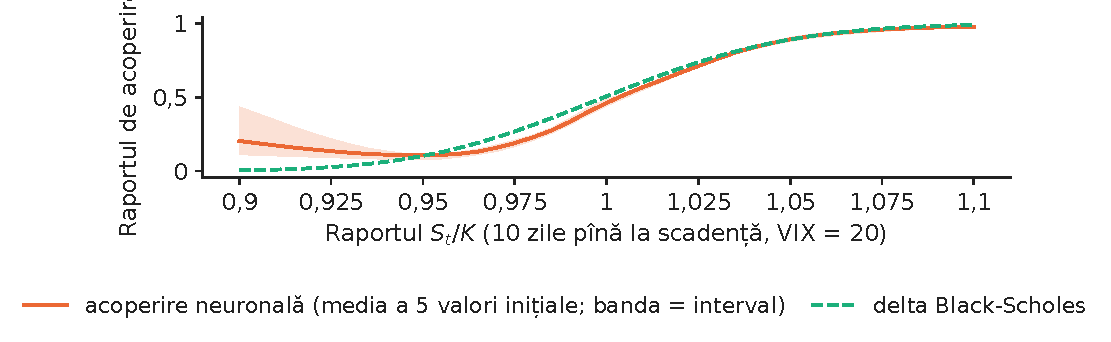
\includegraphics[width=\textwidth,height=0.500\textheight,keepaspectratio]{charts/ro/hedge_delta.pdf}\end{center}\vspace{-3mm}
\chartsource{Sursa: Yahoo Finance, cotații zilnice. Date: politică antrenată pe traiectorii de 21 de zile începute în 2005-2016.}
\vspace{0.5mm}
\begin{itemize}\setlength{\itemsep}{0pt}
  \item La bani: acoperirea neuronală 0{,}46, față de Black-Scholes 0{,}51
    \begin{itemize}\setlength{\itemsep}{0pt}
      \item Banda arată dispersia pe cinci valori inițiale.
    \end{itemize}
\end{itemize}
\par\vfill\noindent{\scriptsize\color{FooterGray}(calcul propriu)}\hfill\qlink{NN\_L10\_hedge\_delta}{Quantlets/L10/NN_L10_hedge_delta}\par\vspace{0.5mm}
\end{frame}

\begin{frame}{Costurile de tranzacționare și avantajul acoperirii învățate}
\small
\intuition{ES$_{95}$ al pierderii din acoperire pentru costuri de la 0 la 50 pb; o rețea antrenată pentru fiecare nivel de cost.}
\begin{center}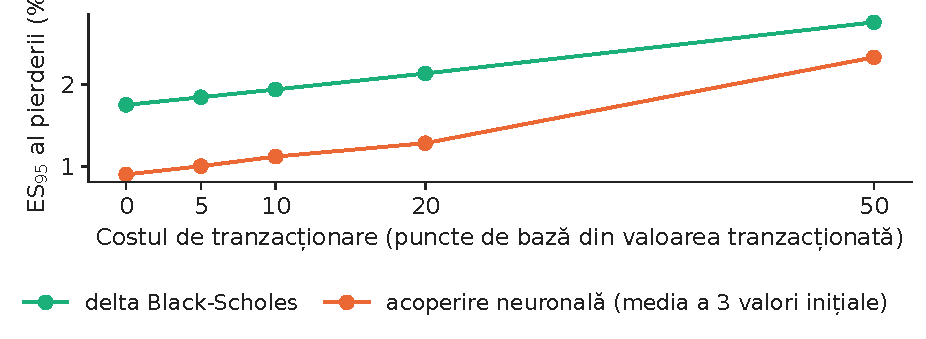
\includegraphics[width=\textwidth,height=0.381\textheight,keepaspectratio]{charts/ro/hedge_costs.pdf}\end{center}\vspace{-3mm}
\chartsource{Sursa: Yahoo Finance, cotații zilnice. Date: traiectorii de test începute 2 ianuarie 2020 - 1 octombrie 2026.}
\vspace{0.5mm}
\begin{itemize}\setlength{\itemsep}{0pt}
  \item Fără cost: delta 1{,}75, acoperire neuronală 0{,}90
    \begin{itemize}\setlength{\itemsep}{0pt}
      \item 50 pb: delta 2{,}76, acoperire neuronală 2{,}34 (\% din indice).
    \end{itemize}
\end{itemize}
\par\vfill\manager{valoarea unei acoperiri învățate crește cu fricțiunile: active suport nelichide, diferențe mari între cotații, acoperiri pe energie și mărfuri.}\par\vspace{0.5mm}
\par\vfill\noindent{\scriptsize\color{FooterGray}(calcul propriu)}\hfill\qlink{NN\_L10\_hedge\_costs}{Quantlets/L10/NN_L10_hedge_costs}\par\vspace{0.5mm}
\end{frame}

\begin{frame}{Reinforcement learning în producție: riscul de model}
\small
\begin{columns}[T,onlytextwidth]
\begin{column}{0.49\textwidth}
\begin{itemize}\setlength{\itemsep}{4pt}
  \item \textbf{Proiectarea recompensei}: agentul optimizează exact ce scrieți
    \begin{itemize}\setlength{\itemsep}{0pt}
      \item Dacă omiteți costurile, riscul sau restricțiile, va exploata lipsa.
    \end{itemize}
  \item \textbf{Diferența față de simulator}: reluarea istorică ignoră impactul propriu asupra prețului și regimurile viitoare.
  \item \textbf{Evaluarea offline}: o singură perioadă de test, folosită o dată
    \begin{itemize}\setlength{\itemsep}{0pt}
      \item Mai multe valori inițiale
      \item Un test față de regula folosită deja.
    \end{itemize}
\end{itemize}
\end{column}
\begin{column}{0.49\textwidth}
\begin{itemize}\setlength{\itemsep}{4pt}
  \item \textbf{Limite de siguranță}: măștile de acțiune (nivelul de încărcare, limitele de poziție), oprirea de urgență, aprobarea umană.
  \item \textbf{Explicabilitate}: un tabel sau o curbă a raportului de acoperire pot fi auditate
    \begin{itemize}\setlength{\itemsep}{0pt}
      \item Cursul 11 explică politicile neuronale.
    \end{itemize}
  \item \textbf{Monitorizare}: comparați lunar rata de captare și volumul tranzacționat cu testul retrospectiv.
\end{itemize}
\end{column}
\end{columns}
\par\vfill\manager{tratați o politică RL ca pe orice model al băncii: documentată, validată independent, monitorizată și cu o regulă de rezervă.}\par\vspace{0.5mm}
\par\vfill\noindent{\scriptsize\color{FooterGray}(Hambly, Xu \& Yang, 2023)}\par\vspace{0.5mm}
\end{frame}

\section*{Recapitulare}

\begin{frame}{Test 1: previziunea perfectă}
\small
\begin{itemize}
  \item Un furnizor arată că agentul său pentru baterie a obținut 95\,\% din venitul programării dinamice într-un test retrospectiv în care DP a folosit chiar prețurile zilei.
    \begin{itemize}\setlength{\itemsep}{0pt}
      \item Ce întrebați?
    \end{itemize}
\end{itemize}
\vspace{2mm}
\begin{exampleblock}{R\u{a}spuns}
\begin{itemize}
  \item Dacă starea agentului conținea prețurile zilei: dacă da, cei 95\,\% provin din informație din viitor
    \begin{itemize}\setlength{\itemsep}{0pt}
      \item Un agent corect vede doar ziua de ieri și este comparat cu planul optim de ieri, ca în testul nostru (DQN 50{,}1\,\%, planul naiv 80{,}7\,\%).
    \end{itemize}
\end{itemize}
\end{exampleblock}
\end{frame}

\begin{frame}{Test 2: plafonarea PPO}
\small
\begin{itemize}
  \item Într-o actualizare PPO, o acțiune are avantajul $\hat A_t>0$, iar noua politică îi dă deja de 1{,}5 ori probabilitatea veche.
    \begin{itemize}\setlength{\itemsep}{0pt}
      \item Ce gradient transmite obiectivul plafonat pentru acest eșantion, cu $\epsilon=0{,}2$?
    \end{itemize}
\end{itemize}
\vspace{2mm}
\begin{exampleblock}{R\u{a}spuns}
\begin{itemize}
  \item Zero: $\rho_t=1{,}5>1+\epsilon$, minimul alege termenul plafonat $1{,}2\,\hat A_t$, care nu depinde de $\btheta$
    \begin{itemize}\setlength{\itemsep}{0pt}
      \item Politica nu mai este împinsă în acest pas.
    \end{itemize}
\end{itemize}
\end{exampleblock}
\end{frame}

\begin{frame}{Test 3: interpretarea unui rezultat de tranzacționare}
\small
\begin{itemize}
  \item Agentul PPO are, pentru cea mai bună valoare inițială, un raport Sharpe de test peste strategia cumpără și păstrează.
    \begin{itemize}\setlength{\itemsep}{0pt}
      \item Intervalul bootstrap al diferenței de raport Sharpe pentru strategia mediată pe valori inițiale este [\ensuremath{-}0{,}08; 0{,}56].
      \item Îl folosiți?
    \end{itemize}
\end{itemize}
\vspace{2mm}
\begin{exampleblock}{R\u{a}spuns}
\begin{itemize}
  \item Nu: cea mai bună valoare inițială este un rezultat selectat, iar un interval care conține zero nu arată o valoare adăugată
    \begin{itemize}\setlength{\itemsep}{0pt}
      \item Păstrați regula simplă.
    \end{itemize}
\end{itemize}
\end{exampleblock}
\end{frame}

\begin{frame}{Recapitulare}
\small
\begin{itemize}\setlength{\itemsep}{4pt}
  \item \textbf{MDP + Bellman}: scrieți starea, acțiunea, recompensa
    \begin{itemize}\setlength{\itemsep}{0pt}
      \item DP rezolvă exact problemele mici și dă plafonul (bateria: 202{,}1 mii EUR pe anii de test).
    \end{itemize}
  \item \textbf{Metode bazate pe valoare}: Q-learning și DQN învață din prețurile de ieri
    \begin{itemize}\setlength{\itemsep}{0pt}
      \item Rate de captare 57{,}0\,\% și 50{,}1\,\%, planul naiv 80{,}7\,\%.
    \end{itemize}
  \item \textbf{Gradientul politicii}: PPO pe S\&P 500 dă un raport Sharpe de 0{,}83, față de 0{,}61 pentru strategia cumpără și păstrează, cu un interval bootstrap care conține zero.
  \item \textbf{Acoperirea neuronală}: ES$_{95}$ al pierderii 1{,}15\,\%, față de 1{,}94\,\% pentru acoperirea delta, la 10 pb.
  \item \textbf{Verdictul pe date reale}: bateria --- regula simplă cîștigă
    \begin{itemize}\setlength{\itemsep}{0pt}
      \item Tranzacționarea --- Sharpe mai mare, dar nesemnificativ
      \item Acoperirea --- politica învățată cîștigă pentru fiecare valoare inițială.
    \end{itemize}
  \item \textbf{Urmează}: cursul 11 deschide cutia neagră: explicarea a ceea ce a învățat o rețea neuronală.
\end{itemize}
\end{frame}

\begin{frame}{Cercetările grupului nostru: stocare, prețuri și învățare automată în finanțele energiei}
\footnotesize
\begin{itemize}\setlength{\itemsep}{4pt}
  \item \textbf{Arbitrajul cu baterii pe piețele pentru ziua următoare}: prognozele probabilistice comune ale vectorului de prețuri orare alimentează decizia de încărcare și descărcare a unei baterii pe piețele din Europa Centrală și de Est
    \begin{itemize}\setlength{\itemsep}{0pt}
      \item Dispecerizarea are nevoie de distribuția comună, nu doar de prețuri punctuale (Andrei, Cepoi, Dumitrescu, Lessmann, Chiriac (Luchian), Pele \& Petukhina, 2026, Social Science Research Network (SSRN) 6872381).
    \end{itemize}
  \item \textbf{Patru generații de modele de preț}: o evaluare comparativă de la modelele statistice la învățarea automată, deep learning și modelele transformer pentru prețurile energiei (Andrei, Velev, Toma, Pele \& Lessmann, 2024, arXiv 2411.03372) --- prognozele de care are nevoie un agent de dispecerizare.
  \item \textbf{Inteligența artificială (AI) în finanțele energiei}: o analiză sistematică a literaturii despre modul în care învățarea automată și reinforcement learning schimbă deciziile de tranzacționare, de risc și de stocare pe piețele de energie (Anagnoste et al., 2025, Energy Strategy Reviews).
\end{itemize}\par\vspace{1mm}{\scriptsize \begin{itemize}
  \item Rezultatele sînt cele din lucrări; cifrele de pe celelalte slide-uri provin din datele noastre.
\end{itemize}}
\par\vfill\noindent{\scriptsize\color{FooterGray}(Academia de Studii Economice din București (ASE); Academia Română, Institutul de Prognoză Economică (IPE))}\par\vspace{0.5mm}
\end{frame}

\begin{frame}{Lecturi și resurse suplimentare}
\small
\begin{columns}[T,onlytextwidth]
\begin{column}{0.5\textwidth}
\begin{itemize}\setlength{\itemsep}{4pt}
  \item \textbf{Sutton \& Barto (2018)}, manualul de referință, gratuit online: \href{http://incompleteideas.net/book/the-book-2nd.html}{incompleteideas.net/book}.
  \item \textbf{Spinning Up in Deep RL} (OpenAI), derivări clare pentru gradienții de politică și PPO: \href{https://spinningup.openai.com}{spinningup.openai.com}.
  \item \textbf{Hambly, Xu \& Yang (2023)}: o sinteză a aplicațiilor RL în finanțe.
\end{itemize}
\end{column}
\begin{column}{0.47\textwidth}
\begin{itemize}\setlength{\itemsep}{4pt}
  \item \textbf{Acest curs}: cod, date, notebook-uri --- \href{https://github.com/danpele/NEURAL_BIZ}{github.com/danpele/NEURAL\_BIZ}.
  \item \textbf{Încercați singuri}: notebooks/L10\_notebook\_ro.ipynb reproduce fiecare metodă din acest curs
    \begin{itemize}\setlength{\itemsep}{0pt}
      \item Seminarul adaugă experimente cu randamentul, dimensiunea bateriei și costurile.
    \end{itemize}
  \item \textbf{Acoperirea neuronală}: Buehler et al.\ (2019), lucrarea din spatele ultimei secțiuni.
\end{itemize}
\end{column}
\end{columns}
\end{frame}

\begin{frame}{Bibliografie (1/2)}
\scriptsize
\begin{itemize}\setlength{\itemsep}{0pt}\scriptsize
\item Andrei, A.-V., Cepoi, C.\,O., Dumitrescu, B.\,A., Lessmann, S., Chiriac (Luchian), A.-C., Pele, D.\,T.\ \& Petukhina, A.\ (2026). Joint probabilistic forecasting for battery arbitrage in day-ahead power markets. SSRN Working Paper 6872381. \href{https://doi.org/10.2139/ssrn.6872381}{doi:10.2139/ssrn.6872381}
\item Anagnoste, S., Andrei, A.-V., Bolovăneanu, V., Cepoi, C.-O., Clodnitchi, R., Cramer, A.-A., Grecu, R.-A., Lessmann, S., Pele, D.\,T., Petukhina, A.\ \& Strat, V.\,A.\ (2025). The role of AI in (re)shaping energy finance: A systematic literature review. \textit{Energy Strategy Reviews}, 61, 101833. \href{https://doi.org/10.1016/j.esr.2025.101833}{doi:10.1016/j.esr.2025.101833}
\item Andrei, A.-V., Velev, G., Toma, F.-M., Pele, D.\,T.\ \& Lessmann, S.\ (2024). Energy price modelling: A comparative evaluation of four generations of forecasting methods. \href{https://arxiv.org/abs/2411.03372}{arXiv:2411.03372}
\item Bellman, R.\ (1957). \textit{Dynamic Programming}. Princeton University Press.
\item Buehler, H., Gonon, L., Teichmann, J.\ \& Wood, B.\ (2019). Deep hedging. \textit{Quantitative Finance}, 19(8), 1271--1291. \href{https://doi.org/10.1080/14697688.2019.1571683}{doi:10.1080/14697688.2019.1571683}
\item Diebold, F.\,X.\ \& Mariano, R.\,S.\ (1995). Comparing predictive accuracy. \textit{Journal of Business \& Economic Statistics}, 13(3), 253--263. \href{https://doi.org/10.1080/07350015.1995.10524599}{doi:10.1080/07350015.1995.10524599}
\item Hambly, B., Xu, R.\ \& Yang, H.\ (2023). Recent advances in reinforcement learning in finance. \textit{Mathematical Finance}, 33(3), 437--503. \href{https://doi.org/10.1111/mafi.12382}{doi:10.1111/mafi.12382}
\item Mnih, V.\ et al.\ (2015). Human-level control through deep reinforcement learning. \textit{Nature}, 518, 529--533. \href{https://doi.org/10.1038/nature14236}{doi:10.1038/nature14236}
\item Moody, J.\ \& Saffell, M.\ (2001). Learning to trade via direct reinforcement. \textit{IEEE Transactions on Neural Networks}, 12(4), 875--889. \href{https://doi.org/10.1109/72.935097}{doi:10.1109/72.935097}
\end{itemize}
\end{frame}

\begin{frame}{Bibliografie (2/2)}
\scriptsize
\begin{itemize}\setlength{\itemsep}{0pt}\scriptsize
\item Politis, D.\,N.\ \& Romano, J.\,P.\ (1994). The stationary bootstrap. \textit{Journal of the American Statistical Association}, 89(428), 1303--1313. \href{https://doi.org/10.1080/01621459.1994.10476870}{doi:10.1080/01621459.1994.10476870}
\item Rockafellar, R.\,T.\ \& Uryasev, S.\ (2000). Optimization of conditional value-at-risk. \textit{Journal of Risk}, 2(3), 21--41. \href{https://doi.org/10.21314/JOR.2000.038}{doi:10.21314/JOR.2000.038}
\item Schulman, J., Moritz, P., Levine, S., Jordan, M.\ \& Abbeel, P.\ (2016). High-dimensional continuous control using generalized advantage estimation. ICLR. \href{https://arxiv.org/abs/1506.02438}{arXiv:1506.02438}
\item Schulman, J., Wolski, F., Dhariwal, P., Radford, A.\ \& Klimov, O.\ (2017). Proximal policy optimization algorithms. \href{https://arxiv.org/abs/1707.06347}{arXiv:1707.06347}
\item Sutton, R.\,S.\ \& Barto, A.\,G.\ (2018). \textit{Reinforcement Learning: An Introduction}, 2nd ed. MIT Press. \href{http://incompleteideas.net/book/the-book-2nd.html}{incompleteideas.net/book}
\item Sutton, R.\,S., McAllester, D., Singh, S.\ \& Mansour, Y.\ (2000). Policy gradient methods for reinforcement learning with function approximation. \textit{Advances in Neural Information Processing Systems}, 12, 1057--1063.
\item van Hasselt, H., Guez, A.\ \& Silver, D.\ (2016). Deep reinforcement learning with double Q-learning. \textit{Proceedings of the AAAI Conference on Artificial Intelligence}, 30(1). \href{https://doi.org/10.1609/aaai.v30i1.10295}{doi:10.1609/aaai.v30i1.10295}
\item Watkins, C.\,J.\,C.\,H.\ \& Dayan, P.\ (1992). Q-learning. \textit{Machine Learning}, 8, 279--292. \href{https://doi.org/10.1007/BF00992698}{doi:10.1007/BF00992698}
\item Williams, R.\,J.\ (1992). Simple statistical gradient-following algorithms for connectionist reinforcement learning. \textit{Machine Learning}, 8, 229--256. \href{https://doi.org/10.1007/BF00992696}{doi:10.1007/BF00992696}
\end{itemize}
\end{frame}

\appendix

\section*{Anexă}

\begin{frame}{Anexa A: convergența Q-learning}
\small
\begin{itemize}\setlength{\itemsep}{3pt}
  \item Operatorul de optimalitate Bellman $(\mathcal{T}Q)(s,a)=R(s,a)+\gamma\E_{s'}\max_{a'}Q(s',a')$ este o $\gamma$-contracție în norma sup: $\|\mathcal{T}Q_1-\mathcal{T}Q_2\|_\infty\le\gamma\|Q_1-Q_2\|_\infty$.
  \item Q-learning este o aproximare stocastică a punctului fix: $Q_{t+1}=(1-\alpha_t)Q_t+\alpha_t(\mathcal{T}Q_t+\varepsilon_t)$, cu zgomot $\varepsilon_t$ de medie zero.
  \item Condițiile Robbins-Monro $\sum_t\alpha_t(s,a)=\infty$, $\sum_t\alpha_t^2(s,a)<\infty$ și vizitele infinite dau $Q_t\to Q^{*}$ aproape sigur (Watkins \& Dayan, 1992).
  \item Cu $\gamma=1$ pe un orizont finit, argumentul contracției este înlocuit de inducția înapoi pe cei 24 de pași.
  \item Un $\alpha=0{,}05$ constant (ca aici) converge doar într-o vecinătate a lui $Q^{*}$
    \begin{itemize}\setlength{\itemsep}{0pt}
      \item Setul de validare alege cea mai bună epocă.
    \end{itemize}
\end{itemize}
\par\vfill\noindent{\scriptsize\color{FooterGray}(Watkins \& Dayan, 1992; Sutton \& Barto, 2018, ch.\ 6)}\par\vspace{0.5mm}
\end{frame}

\begin{frame}{Anexa B: setările celor trei agenți}
\footnotesize
{\footnotesize\renewcommand{\arraystretch}{1.05}\setlength{\tabcolsep}{4pt}
\begin{tabular}{@{}p{0.24\textwidth}p{0.22\textwidth}p{0.24\textwidth}p{0.24\textwidth}@{}}\toprule
Setare & Q-learning / DQN & PPO & Acoperire neuronală \\ \midrule
Rețea & tabel; 2$\times$128 ReLU & 2$\times$64 tanh, comun & 2$\times$32 ReLU, sigmoid \\
Optimizator & $\alpha=0{,}05$; Adam $3\cdot10^{-4}$ & Adam $3\cdot10^{-4}$ & Adam $3\cdot10^{-3}$ \\
Actualizare / orizont & $\gamma=1$, 24 h & $\gamma=0{,}99$, $\lambda=0{,}95$, 126 z & 21 de zile \\
Explorare & $\varepsilon$: 1 $\to$ 0{,}05 & entropie 0{,}01 & -- \\
Bugetul de antrenare & 40 de epoci; 40 de actualizări de 512 pe oră & 150 de iterații $\times$ 64 de episoade & 600 de pași pe tot setul \\
Selecție & cel mai bun venit în 2024 & cel mai bun Sharpe 2017--2019 & fără (buget fix) \\
Timp de rulare (5 valori) & 1\,838 s & 160 s & 728 s \\
\bottomrule\end{tabular}}
\par\vfill\noindent{\scriptsize\color{FooterGray}(calcul propriu)}\hfill\tryit{notebook \S3--\S6}\par\vspace{0.5mm}
\end{frame}

\begin{frame}{Anexa C: estimatorul generalizat al avantajului}
\small
\begin{itemize}\setlength{\itemsep}{3pt}
  \item Avantajul pe $k$ pași: $\hat A_t^{(k)}=\sum_{l=0}^{k-1}\gamma^{l}r_{t+l+1}+\gamma^{k}V(s_{t+k})-V(s_t)=\sum_{l=0}^{k-1}\gamma^{l}\delta_{t+l}$.
  \item GAE este media ponderată exponențial $(1-\lambda)\sum_{k\ge1}\lambda^{k-1}\hat A_t^{(k)}=\sum_{l\ge0}(\gamma\lambda)^{l}\delta_{t+l}$.
  \item Se calculează înapoi într-o singură trecere: $\hat A_t=\delta_t+\gamma\lambda\hat A_{t+1}$, $\hat A_T=0$ (bucla din analysis\_L10.py).
  \item Compromisul deplasare-varianță: un $\lambda$ mic are încredere în critic (deplasat dacă $V$ este greșit), un $\lambda$ mare în recompensele eșantionate (zgomotos).
\end{itemize}
\par\vfill\noindent{\scriptsize\color{FooterGray}(Schulman et al., 2016)}\par\vspace{0.5mm}
\end{frame}

\end{document}
